\documentclass[12pt, a4paper]{article}

\usepackage[utf8]{vietnam}  % Vietnamese input
\usepackage{tikz}           % titlepage border
\usetikzlibrary{calc}       % titlepage border
\usepackage{niceframe}      % For titlepage

\usepackage{array}          % For side by side comparisions
\usepackage{lipsum}         % For text generation

%\usepackage{graphicx}      %  Use this if you want more control over \includegraphics{}

\usepackage{fancyhdr}       % For header and footer

\usepackage{hyperref}       % For hypertext inserting

\usepackage{times}
\usepackage{fancyhdr,graphicx,amsmath,amssymb}
\usepackage[ruled,vlined]{algorithm2e}


%For code presentation
\usepackage{listings}
\usepackage{color}
\definecolor{dkgreen}{rgb}{0,0.6,0}
\definecolor{gray}{rgb}{0.5,0.5,0.5}
\definecolor{mauve}{rgb}{0.58,0,0.82}

\lstset{frame=tb,
  language=Python,
  aboveskip=3mm,
  belowskip=3mm,
  showstringspaces=false, 
  columns=flexible,
  basicstyle={\small\ttfamily},
  numbers=none,
  numberstyle=\tiny\color{gray},
  keywordstyle=\color{blue},
  commentstyle=\color{dkgreen},
  stringstyle=\color{mauve},
  breaklines=true,
  breakatwhitespace=true,
  tabsize=3
}
% For code presentation


%For fixed table postition
\usepackage{float}

%For section size
\usepackage{titlesec}

\titleformat*{\section}{\LARGE\bfseries}
\titleformat*{\subsection}{\Large\bfseries}
\titleformat*{\subsubsection}{\large\bfseries}

\lstdefinestyle{mystyle}{
    breakatwhitespace=false,         
    breaklines=true,                 
    captionpos=b,                    
    keepspaces=true,                 
    numbers=left,                    
    numbersep=5pt,                  
    showspaces=false,                
    showstringspaces=false,
    showtabs=false,                  
    tabsize=4,
}

\lstset{style=mystyle}


\usepackage[a4paper, total={6in, 8in}]{geometry}
\newcommand\tab[1][0.5cm]{\hspace*{#1}}


%TitlePage

\begin{document}
\include{pythonlisting}

\begin{titlepage}
    \begin{tikzpicture}[remember picture,overlay,inner sep=0,outer sep=0]
        \draw[blue!70!black,line width=4pt] ([xshift=-1.5cm,yshift=-2cm]current page.north east) coordinate (A)--([xshift=1.5cm,yshift=-2cm]current page.north west) coordinate(B)--([xshift=1.5cm,yshift=2cm]current page.south west) coordinate (C)--([xshift=-1.5cm,yshift=2cm]current page.south east) coordinate(D)--cycle;

        \draw ([yshift=0.5cm,xshift=-0.5cm]A)-- ([yshift=0.5cm,xshift=0.5cm]B)--
        ([yshift=-0.5cm,xshift=0.5cm]B) --([yshift=-0.5cm,xshift=-0.5cm]B)--([yshift=0.5cm,xshift=-0.5cm]C)--([yshift=0.5cm,xshift=0.5cm]C)--([yshift=-0.5cm,xshift=0.5cm]C)-- ([yshift=-0.5cm,xshift=-0.5cm]D)--([yshift=0.5cm,xshift=-0.5cm]D)--([yshift=0.5cm,xshift=0.5cm]D)--([yshift=-0.5cm,xshift=0.5cm]A)--([yshift=-0.5cm,xshift=-0.5cm]A)--([yshift=0.5cm,xshift=-0.5cm]A);


        \draw ([yshift=-0.3cm,xshift=0.3cm]A)-- ([yshift=-0.3cm,xshift=-0.3cm]B)--
        ([yshift=0.3cm,xshift=-0.3cm]B) --([yshift=0.3cm,xshift=0.3cm]B)--([yshift=-0.3cm,xshift=0.3cm]C)--([yshift=-0.3cm,xshift=-0.3cm]C)--([yshift=0.3cm,xshift=-0.3cm]C)-- ([yshift=0.3cm,xshift=0.3cm]D)--([yshift=-0.3cm,xshift=0.3cm]D)--([yshift=-0.3cm,xshift=-0.3cm]D)--([yshift=0.3cm,xshift=-0.3cm]A)--([yshift=0.3cm,xshift=0.3cm]A)--([yshift=-0.3cm,xshift=0.3cm]A);

    \end{tikzpicture}



    \centerline{\textbf{\LARGE{University of Science}}}
    \bigskip
    \centerline{\LARGE{Viet Nam National University - Ho Chi Minh city}}

    \centerline{\huge{--------------------------------------}}

    \centerline{
\includegraphics[width=40mm]{logo.jpg}}

    \centerline{\niceframe[14cm]
        {
            \begin{center}
                \LARGE{\textbf{Final Project}}
                \linebreak
                \centering\huge{\textbf{VẬT LÝ CHO CÔNG NGHỆ THÔNG TIN}}
            \end{center}
        }
    }
    \raggedright
    \bigskip
    \begin{center}
        \begin{table}[h]
            \begin{tabular}{rrlc}
                 & \large{\textbf{Giảng viên lý thuyết}} & \large{Cao Xuân Nam}      &          \\ \\
                 & \large{\textbf{Giảng viên thực hành}} & \large{Đặng Hoài Thương}  &          \\ \\
                 & \large{\textbf{Sinh viên}}        & \large{Lê Hoàng Sang}        & \large{21127158}  \\ \\
                 & \large{\textbf{}}                 & \large{Vũ Đình Chương}       & \large{21127236}  \\ \\
                 & \large{\textbf{}}                 & \large{Nguyễn Quốc Huy}      & \large{21127511}  \\ \\
            \end{tabular}
        \end{table}
    \end{center}
\end{titlepage}



%Header&Footer

\pagestyle{fancy}
\fancyhf{}
\addtolength{\topmargin}{-0.70894pt}
\setlength{\headheight}{12.70894pt}

\lhead{\textbf{FIT-HCMUS}}
\rhead{\textbf{Internet of things}}
\rfoot{\textbf{\thepage}}

%rename content table
\renewcommand*{\contentsname}{Mục lục}
\tableofcontents

\pagebreak

\section{LỜI NÓI ĐẦU}
\begin{itemize}
    \item Đây là dự án phục vụ cho môn Vật lý cho Công nghệ thông tin (Internet of things). 
    Trong dự án có áp dụng tất cả những kiến thức cũng như các thiết bị đã được dạy bởi môn học. 
    Ngoài ra, nhằm đáp ứng cho các yêu cầu khách quan trong đời sống, nhóm cũng đưa vào một số thiết bị mới nhưng quen thuộc với cuộc sống. 
    Dự án hướng đến mục đích bảo vệ và phục hồi tài nguyên nên năng lượng cần cung cấp cho máy là năng lượng sạch lấy từ thiên nhiên.
    \item Các thành viên trong nhóm gồm có:
    \begin{table}[htp]
        \centering
        \begin{tabular}{|c|c|l|}
        \cline{1-3}
        MSSV     & Họ tên            &  Vai trò \\ \cline{1-3} 
        21127158 & Lê Hoàng Sang     &  Node-red, các xử lí trên website\\ \cline{1-3}
        21127236 & Vũ Đình Chương    &  Lập trình mạch điện, gửi thông báo\\ \cline{1-3}
        21127511 & Nguyễn Quốc Huy   &  Vẽ 3D, lập trình mạch điện\\ \cline{1-3} 
        \end{tabular}
    \end{table}
    \item Quy mô của dự án hiện đang ở mức giả lập, đến từ khoa Công nghệ thông tin, Trường Đại học Khoa học Tự nhiên.
\end{itemize}
\section{TỔNG QUAN}

\subsection{Tên đề tài}
\begin{center}
    \textcolor{red}{\Large\textbf{{THÙNG XỬ LÍ RÁC THÔNG MINH}}}
\end{center}
\subsection{Lý do chọn đề tài}
\begin{itemize}
    \item Rác thải sinh hoạt hàng ngày của mỗi gia đình phần lớn là rác hữu cơ. 
Nếu có thể tận dụng nguồn rác này để làm phân bón thì có thể giảm tải rất lớn cho việc xử lí rác cho các nhà máy và góp phần đáng kể cho việc bảo vệ môi trường. 
Chính vì vậy, chúng em nghiên cứu chế tạo một sản phẩm là “Thùng xử lí rác thông minh”.
    \item Sản phẩm sử dụng men vi sinh kết hợp với ứng dụng năng lượng mặt trời trong quá trình xử lí rác do đó tiết kiệm được tài nguyên, tạo ra phân hữu cơ, giảm ô nhiễm môi trường, mang lại lợi ích cho gia đình và cộng đồng.
\end{itemize}

\subsection{Vấn đề đặt ra}

\begin{itemize}
    \item \textbf{Vì sao lại sử dụng năng lượng mặt trời?}
    \begin{itemize}
        \item Đây là nguồn năng lượng tái tạo không bị cạn kiệt, có thể đáp ứng nhu cầu sử dụng của tất cả mọi người một cách liên tục. 
        \item Có thể sử dụng ở bất cứ đâu có ánh nắng mặt trời chiếu sáng, vào ban đêm có thể dùng pin dự trữ từ buổi sáng. 
        \item Năng lượng mặt trời là nguồn năng lượng sạch có sẵn trong tự nhiên và không gây ô nhiễm môi trường. 
        \item Do thùng rác thiết kế có sử dụng điện và chỉ có điện mặt trời mới có thể đáp ứng tính linh động của việc đặt vị trí thùng rác ở các nơi khác nhau.
        \item Hiệu quả sử dụng cao với chi phí đầu vào thấp. 
    \end{itemize}
    \item \textbf{Vì sao lại là thùng ủ phân bón?}
    \begin{itemize}
        \item Do tính tiện lợi, tiết kiệm thời gian, chi phí và công sức.
        \item Đảm bảo an toàn và hợp vệ sinh.
        \item Sử dụng nguồn năng lượng sạch.
        \item Phân bón được ủ bằng thùng rác ủ phân chuyên dụng sẽ tạo ra sản phẩm là chất mùn ổn định thu được từ quá trình phân hủy các chất hữu cơ, không chứa các mầm bệnh, không lôi kéo các côn trùng (do là quy trình khép kín), được lưu trữ an toàn.
        \item Có lợi cho sự phát triển của cây trồng: cung cấp chất dinh dưỡng cho cây.
        \item Tăng đồ phì nhiêu cho đất.
        \item Nếu mô hình ủ rác hữu cơ thành phân bón được nhân rộng, việc phân loại và sử dụng men vi sinh phân hủy rác sẽ giúp giảm thiểu đáng kể nguồn gây ô nhiễm môi trường; đồng thời, góp phần xây dựng nền nông nghiệp tiết kiệm, an toàn và bền vững.
    \end{itemize}
    \item \textbf{Áp dụng vào môn học như thế nào?} 
    \begin{itemize}
        \item Vận dụng kiến thức lập trình IoT, mạch điện Arduino và các thiết bị điện tử liên quan. 
        \item Tạo ra một dự án thiết thực, tính ứng dụng và giúp ích cho cộng đồng cao. 
    \end{itemize}
\end{itemize}

\subsection{Đặc điểm và lợi ích}
\begin{itemize}
    \item Có thể kiểm tra tiến độ và trạng thái của thùng ủ qua website. 
    \item Vì dùng bằng năng lượng mặt trời nên tiết kiệm chi phí điện năng tiêu thụ cho hộ gia đình.
    \item Linh động việc đặt ở các vị trí khác nhau có ánh sáng mặt trời.
    \item Thời gian sử dụng lâu dài, không phải tốn sức vận hành.
    \item Sản phẩm giúp ủ rác thải sinh hoạt (rác thải hữu cơ) tại nhà nên có được một nguồn phân bón liên tục cung cấp cho cây trồng. Đồng thời giảm lượng rác thải ra môi trường bên ngoài và giảm chi phí xử lí rác thải của nhà nước.
    \item Tiết kiệm được chi phí mua phân bón cho cây cảnh, trồng trọt.
\end{itemize}

\subsection{Mục tiêu và ý nghĩa}
\begin{itemize}
    \item Tạo ra một dự án có tính ứng dụng cao. 
    \item Góp phần vào lĩnh vực công nghệ thân thiện với môi trường. 
    \item Đưa ra một giải pháp tiện dụng, linh hoạt, tiết kiệm cho các hộ gia đình. 
    \item Sử dụng các linh kiện giá rẻ, dễ tiếp cận đối với các gia đình phổ thông. 
\end{itemize}

\section{CẤU TẠO VÀ THIẾT KẾ}
\subsection{Danh sách thiết bị cần dùng}

\begin{table}[H]
    \centering
    \begin{tabular}{| p{0.05\linewidth}| p{0.3\linewidth}| p{0.1\linewidth}| p{0.15\linewidth}| p{0.15\linewidth}| p{0.20\linewidth}|} \cline{1-6}
    STT & \centering{Tên thiết bị} & \centering{Số lượng} & \centering{Đơn giá} & \centering{Thành tiền} & Đường dẫn\\ \cline{1-6}
    1 & Mạch arduino R3 & \centering{1} & 199000 & 199000 & \href{https://shopee.vn/product/144259413/2642081316?gclid=CjwKCAjw2K6lBhBXEiwA5RjtCbTJV4TKxhrAyMfeYOUDQwQR52w-R9cNOtDFLPn-jTPIaWpPXZtguRoCrVMQAvD_BwE}{Mạch arduino R3} \\ \cline{1-6}
    2 & Module ESP8266 ESP-01 & \centering{1} & 45000 & 45000 & \href{https://banlinhkien.com/module-wifi-esp8266-esp01-p6652259.html}{Module ESP8266 ESP-01} \\ \cline{1-6}
    3 & Động cơ DC 12V giảm tốc & \centering{1} & 99000 & 99000 & \href{https://shopee.vn/product/104103144/5453707854?gclid=CjwKCAjw2K6lBhBXEiwA5RjtCdoA5-9pC6vOUobxaDLcFjmtsYVAaiLZWnn4vBP2DAlsm3I4WXqEuRoCN-UQAvD_BwE}{Động cơ DC 12V giảm tốc} \\ \cline{1-6}
    4 & Cảm biến nhiệt độ, độ ẩm DHT11 & \centering{1} & 35000 & 35000 &  \href{https://shopee.vn/product/185189131/3600332444?gclid=CjwKCAjw2K6lBhBXEiwA5RjtCfJ_-PD2oz3EneuJU14CIIa0qBJT8SXKXSysUuzEtJKVQX-ngxUwxRoCs2wQAvD_BwE}{Cảm biến nhiệt độ, độ ẩm DHT11} \\ \cline{1-6}
    5 & Đèn dây tóc 12V & \centering{1} & 25000 & 25000 & \href{https://shopee.vn/product/14997304/6438455192?gclid=CjwKCAjw2K6lBhBXEiwA5RjtCXhUBhliEga0DGUji7OPtcO9pdM147svoeO5zqeMxV0MC9kwJUDn3xoCEU0QAvD_BwE}{Đèn dây tóc 12V } \\ \cline{1-6}
    6 & Động cơ servo MG996R nhông và bánh răng & \centering{4} & 66000 & 264000 & \href{https://www.lazada.vn/products/dong-co-servo-mg996r-nhong-va-banh-rang-full-kim-loai-i1026138304-s3435872717.html?from_gmc=1&exlaz=d_1:mm_150050845_51350205_2010350205::12:17859528228!!!!!c!!3435872717!240019841&gclid=CjwKCAjw2K6lBhBXEiwA5RjtCcO5LgkSvD-O_FlE8RcZdrekWWcBMOS1Qgnyf2-pBC5ZZ3SYQjT9ahoCvB4QAvD_BwE}{Động cơ servo MG996R nhông và bánh răng} \\ \cline{1-6}
    7 & Tấm pin năng lượng mặt trời 12V - 50W, diện tích 60x80 cm & \centering{1} & 500000 & 500000 & \href{https://www.lazada.vn/products/tam-pin-nang-luong-mat-troi-cong-usb-dau-ra-kep-50w-12v24v-chi-hoac-bo-tam-nang-luong-mat-troi-voi-bo-dieu-khien-10a-i1320954768-s5252422197.html?c=&channelLpJumpArgs=&clickTrackInfo=query%253Apin%252Bn%2525C4%252583ng%252Bl%2525C6%2525B0%2525E1%2525BB%2525A3ng%252Bm%2525E1%2525BA%2525B7t%252Btr%2525E1%2525BB%25259Di%252B12v%252B50w%253Bnid%253A1320954768%253Bsrc%253ALazadaMainSrp%253Brn%253A7649cdbfed011e8b11e432f33225212b%253Bregion%253Avn%253Bsku%253A1320954768_VNAMZ%253Bprice%253A459000%253Bclient%253Adesktop%253Bsupplier_id%253A100015419%253Bpromotion_biz%253A%253Basc_category_id%253A12909%253Bitem_id%253A1320954768%253Bsku_id%253A5252422197%253Bshop_id%253A331&fastshipping=0&freeshipping=0&fs_ab=2&fuse_fs=0&lang=vi&location=N%C6%B0%E1%BB%9Bc%20ngo%C3%A0i&price=4.59E%205&priceCompare=&ratingscore=4.8&request_id=7649cdbfed011e8b11e432f33225212b&review=5&sale=25&search=1&source=search&spm=a2o4n.searchlist.list.11&stock=1}{Tấm pin năng lượng mặt trời} \\ \cline{1-6}
    8 & Dụng cụ trộn & \centering{1} &  50000 & 50000 & - \\ \cline{1-6}
    9 & Module Relay 5V & \centering{1} & 20000 & 20000 & \href{https://shopee.vn/product/50091114/5552205506?gclid=CjwKCAjw2K6lBhBXEiwA5RjtCROnQXSknRS5Mn6qteB8g6c93j0GdO7amSumGPVwoALvy8YZexUnfxoCLuAQAvD_BwE}{Module Relay 5V} \\ \cline{1-6}
    10 & LED LCD 1602 & \centering{1} & 35000 & 35000 & \href{https://shopee.vn/product/52631548/4916526520?gclid=CjwKCAjw2K6lBhBXEiwA5RjtCfnUF2zZcUOhMaJKw7xxskTb0ziaJ7Ld5N0wkaLD0PQ0Tsm6KkSxORoC_qoQAvD_BwE}{LED LCD 1602} \\ \cline{1-6}
    11 & Men ủ EMUNIV & \centering{1} & 33000 & 33000 & \href{https://nongnghieppho.vn/products/che-pham-u-phan-va-rac-thai-emuniv?variant=1039084926&source=googleshop&utm_campaign=pmax&utm_source=googleshop&utm_source=GgAds&utm_medium=cpa&utm_campaign=ggShopping&utm_term=22072022-Smart-HCM-HN-DN&ref=haraads&utm_campaign=haraads&utm_medium=paid&utm_source=google&gclid=CjwKCAjw2K6lBhBXEiwA5RjtCZ774YOCeJ031WhPH-GFsjWj0wOVuUh5qCWrUCqjSAwAUq4qSzbsphoCZFIQAvD_BwE}{Men ủ EMUNIV} \\ \cline{1-6}
    12 & Ắc quy 12V & \centering{1} & 400000 & 400000 & \href{https://shopee.vn/product/70713800/11611368815?gclid=CjwKCAjw2K6lBhBXEiwA5RjtCYjPxO5TLbxeGmb7EHRxVX2JNGEDqyKPMvOrUW2nfQPvYyCM9lc5HxoCkPAQAvD_BwE}{Ắc quy 12V} \\ \cline{1-6}
    13 & Button & \centering{4} & 10000 & 40000 & \href{https://www.lazada.vn/products/combo-10-nut-nhan-4-chan-6x6x5mm-i1504431645-s6303036923.html?from_gmc=1&exlaz=d_1:mm_150050845_51350205_2010350205::12:17916655101!!!!!c!!6303036923!436062007&gclid=CjwKCAjw2K6lBhBXEiwA5RjtCVc2YsdrV1aJB66Ubjqp66X3_-YxMQwaSWF7sYNOiV_P2oiooniMERoCPcAQAvD_BwE}{Button} \\ \cline{1-6}
    14 & Buzzer & \centering{1} & 24000 & 24000 & \href{https://tiki.vn/search?q=c%C3%B2i%20buzzer%205v}{Buzzer}  \\ \cline{1-6}
    15 & Dây cắm & \centering{40} & 5600 & 224000 & \href{https://hshop.vn/collections/day-cam-breadboard-connector}{Dây cắm} \\ \cline{1-6}
    16 & Hộc đựng & \centering{3} & 50000 & 150000 & \href{https://shopee.vn/product/144259413/2642081316?gclid=CjwKCAjw2K6lBhBXEiwA5RjtCbTJV4TKxhrAyMfeYOUDQwQR52w-R9cNOtDFLPn-jTPIaWpPXZtguRoCrVMQAvD_BwE}{Hộc đựng} \\ \cline{1-6}
    17 & Máy xay & \centering{1} & 220000 & 220000 & \href{https://shopee.vn/product/322715332/8475881625?gclid=CjwKCAjw-7OlBhB8EiwAnoOEkzIISACWZinpVm9IpHUbMwxFQXxEZdZfz-PhhBTrL9Pge3VoifNblBoCk6AQAvD_BwE}{Máy xay} \\ \cline{1-6}
    18 & \textbf{TỔNG}  & \centering{-} & - & \textbf{1550000} & - \\ \cline{1-6}
    \end{tabular}
\end{table}
\begin{itemize}
    \item \textbf{Chế phẩm vi sinh sử dụng trong quá trình xử lý rác:} \\ 
    Hiện nay có nhiều chế phẩm sinh học được dùng trong quá trình ủ rác, cây xanh,... cũng như xử lí nước thải thành phân hữu cơ. Nhóm chúng em chọn chế phẩm vi sinh Emuniv trong xử lí rác thải vì dễ tìm, phạm vi áp dụng rộng và giá thành phù hợp.\\
    \centerline{
\includegraphics[scale = 1.2]{Pic/Visinh.jpg}}
    \item \textbf{Bộ phận xay rác hữu cơ:} \\
    Thành phần chính là một máy xay các loại rác hữu cơ, được đấu nối cơ khí và vận hành nhờ một động cơ DV 12V giảm tốc (60 vòng/phút).\\
    \centerline{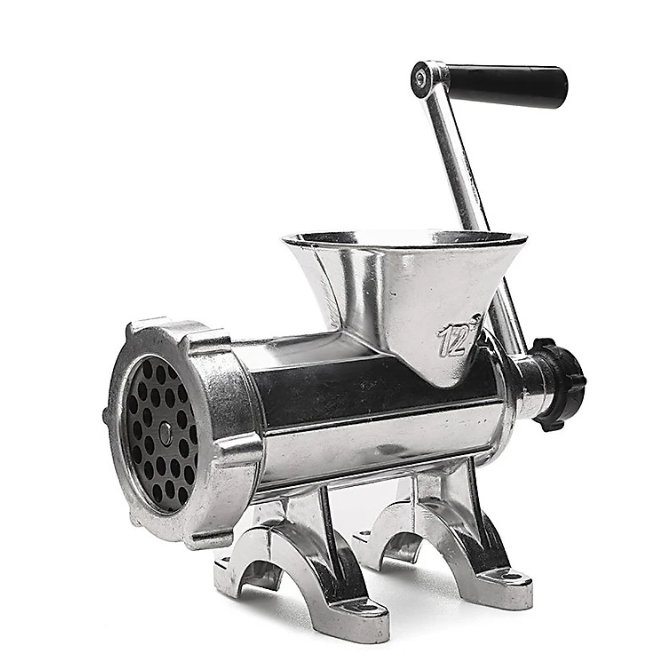
\includegraphics[scale= 0.8]{Pic/Mayxay.png}}
\end{itemize}

\section{NGUYÊN LÝ VÀ CHI TIẾT}
\subsection{Nguyên lý làm việc}
\textbf{Nguyên lý chung của máy có thể hiểu đơn giản như sau:}\\
\centerline{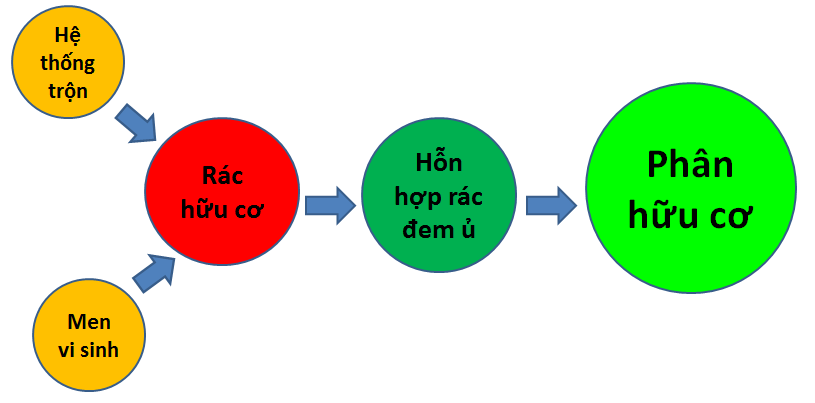
\includegraphics[scale = 0.8]{Pic/Quytrinh.png}} % thêm web
\begin{itemize}
    \item Bước 1: Trộn hỗn hợp rác hữu cơ và lượng men vi sinh đã tính toán trước bằng hệ thống trộn để ra hỗn hợp giữa rác và men.
    \item Bước 2: Ủ hỗn hợp rác hữu cơ và men trong một khoảng thời gian.
    \item Bước 3: Sau khi ủ hỗn hợp rác hữu cơ và men, sau một khoảng thời gian sẽ hình thành phân hữu cơ là thành phẩm. Quá trình này có thể điều khiển từ xa thông qua website.
\end{itemize}

\subsection{Chi tiết hoạt động}
\centerline{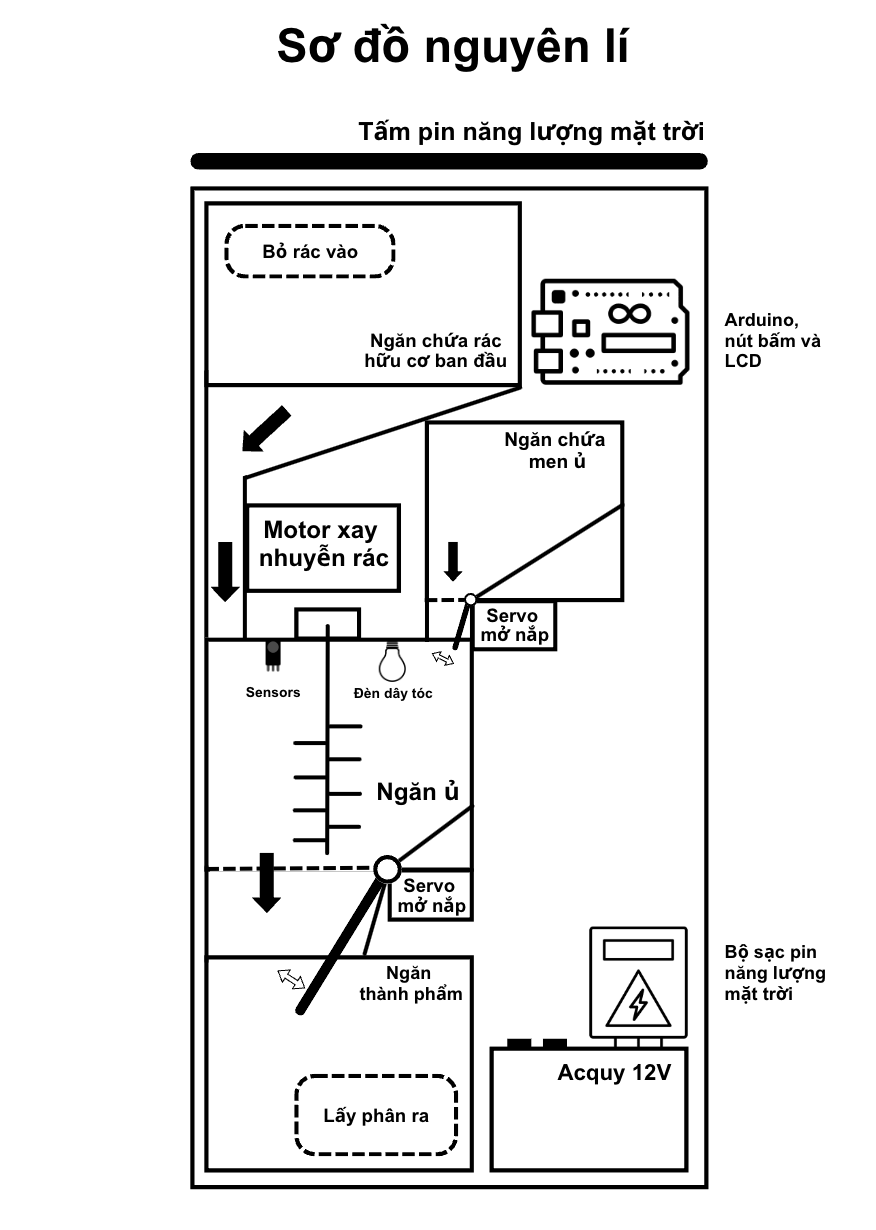
\includegraphics[scale = 1.0]{Pic/image.png}}

\begin{itemize}
    \item Thùng xử lý sẽ nhận năng lượng điện từ tấm pin năng lượng mặt trời, lượng điện năng được chuyển hóa sẽ được lưu trữ vào acquy.
    \item Người sử dụng đầu tiên cần bấm nút nguồn để khởi động.
    \item Người dùng được yêu cầu chọn các chế độ tùy theo khối lượng rác khác nhau (khối lượng rác khác nhau ảnh hưởng đến khối lượng men vi sinh cần thiết). Hoặc điều khiển từ xa thông qua website (Start, chọn chế độ khối lượng/ Pause).
    \item Sau đó, người dùng bấm nút Start để bắt đầu quy trình.
    \item Người dùng có thể kích hoạt từ xa thông qua website Node-red bằng việc chọn thông số khối lượng và Start/Pause thiết bị. Ngoài ra, trong quá trình hoạt động, các thông số như nhiệt độ, độ ẩm, các thông báo, thông báo khẩn cấp luôn được gửi lên website và hiển thị để người dùng theo dõi.
    \item Rác được bỏ vào ngăn đầu tiên là ngăn chờ, từ mức khối lượng người dùng chọn, ta ước lượng được lượng vi sinh cần thiết để ủ.
    \item Sau đó, rác sẽ được đẩy qua ngăn ủ bên dưới bởi bộ phận xay nhuyễn.
    \item Thời gian ủ có thể từ 5 đến 7 ngày để hoàn toàn được trở thành phân hữu cơ, trong khi ủ, có motor trộn để phân được ủ đều.
    \item Trong trường hợp thùng đang có rác hữu cơ đang trong quá trình ủ, phần ngăn chờ bên trên còn có khả năng chứa, rác vẫn được đẩy vào ngăn chờ và quá trình sẽ lặp lại khi người dùng lấy phân cũ ra và ấn Start.
    \item Nếu phân ủ bên dưới đã đến mốc thời gian hoàn thành, thùng sẽ báo trạng thái cho người dùng.
    \item Sau khi ủ thành phân hữu cơ, phân sẽ được đẩy qua ngăn dưới cùng - ngăn thành phẩm, đây là ngăn rời nên người dùng có thể dễ dàng thu nhận phân bón.
    \item Người dùng có thể xem lại lịch sử các phiên hoạt động của thùng rác thông qua tab History của website, thông tin này được lưu trên cloud ThingSpeak.
\end{itemize}

\subsection{Các thông số}

\begin{itemize}
    \item Khi rác vừa được bỏ vào và chạy, máy sẽ xác nhận bằng âm thanh từ Buzzer.
    \item Trong quá trình ủ, LCD sẽ báo trạng thái hoàn thành của thùng, gồm: phần trăm ủ hoàn thành (dựa trên nhiệt độ, ánh sáng, độ ẩm và khối lượng rác người dùng nhập vào), thời gian ước tính còn lại.
    \item Khi người dùng bấm nút chuyển chế độ hiển thị, trên LCD sẽ đổi thông số hiển thị như thời gian, nhiệt độ hay độ ẩm trong thùng ủ.
    \item Ngoài ra, hệ thống còn hỗ trợ người dùng dừng tiến trình, Pause ở cả trên thiết bị và website.
    \item Tất cả các thông số về độ ẩm, thời gian, phần trăm đều sẽ được nêu cụ thể qua website. 
\end{itemize}


\section{KẾ HOẠCH CHI TIẾT}
\pagenumbering{gobble}
\begin{table}[!H]
    \begin{tabular}{|c|c|c|p{0.3\linewidth}|c|c|c|c|} \cline{1-6}
    \textbf{STT} & \centering{\textbf{Bắt đầu}} & \centering{\textbf{Kết thúc}} & \centering{\textbf{Công việc}} & \textbf{Thực hiện} & \textbf{Ghi chú} \\ \cline{1-6} \cline{1-6} 
    
    1 & \centering{20/7/2023} & \centering{30/7/2023} & \centering{Thiết kế mạch điện trên wokwi} & Đình Chương &  \\ \cline{1-6}
    
    2 & \centering{8/8/2023} & \centering{10/8/2023} & \centering{Lấy thời gian thực trên mạch} & Đình Chương &  \\ \cline{1-6}

    3 & \centering{15/8/2023} & \centering{17/8/2023} & \centering{Đẩy thông tin lên website (dạng JSON)} & Đình Chương &  \\ \cline{1-6}

    4 & \centering{20/7/2023} & \centering{21/8/2023} & \centering{Xử lý logic, các tình huống khẩn câp} & Đình Chương &  \\ \cline{1-6}

    5 & \centering{11/8/2023} & \centering{15/8/2023} & \centering{Gửi thông báo qua điện thoại} & Đình Chương &  \\ \cline{1-6}

    6 & \centering{11/8/2023} & \centering{15/8/2023} & \centering{Gửi thông tin từ mạch lên cloud} & Đình Chương &  \\ \cline{1-6}
    
    7 & \centering{17/8/2023} & \centering{23/8/2023} & \centering{Kiểm thử, chạy website} & Đình Chương &  \\ \cline{1-6}

    8 & \centering{17/7/2023} & \centering{23/8/2023} & \centering{Báo cáo chi tiết} & Đình Chương &  \\ \cline{1-6}

    9 & \centering{24/7/2023} & \centering{30/7/2023} & \centering{Cài đặt và xử lý và hiện thông tin lên LCD cho người dùng} & Quốc Huy &  \\ \cline{1-6}

    10 & \centering{30/7/2023} & \centering{15/8/2023} & \centering{Phác thảo chi tiết mô hình 3D (tổng thể và từng phần)} & Quốc Huy &  \\ \cline{1-6}

    11 & \centering{30/7/2023} & \centering{7/8/2023} & \centering{Lập trình kết nối Wifi} & Quốc Huy &  \\ \cline{1-6}
    
    12 & \centering{30/7/2023} & \centering{15/8/2023} & \centering{Nhận thông tin từ website} & Quốc Huy &  \\ \cline{1-6}
    
    13 & \centering{24/7/2023} & \centering{15/8/2023} & \centering{Điều khiển các thiết bị theo logic hệ thống (Servo, Lcd, Relay)} & Quốc Huy &  \\ \cline{1-6}
    
    14 & \centering{24/7/2023} & \centering{7/8/2023} & \centering{Tính toán lượng pin, lượng men và phần trăm hoàn thành} & Quốc Huy &  \\ \cline{1-6}
    
    15 & \centering{17/8/2023} & \centering{23/8/2023} & \centering{Kiểm thử, chạy website} & Quốc Huy &  \\ \cline{1-6}
    
    16 & \centering{17/8/2023} & \centering{23/8/2023} & \centering{Báo cáo chi tiết} & Quốc Huy &  \\ \cline{1-6}
    
    17 & \centering{24/7/2023} & \centering{10/8/2023} & \centering{Thiết kế toàn bộ website (login, trang thông số, login, điều khiển, thông báo...)} & Hoàng Sang &  \\ \cline{1-6}

    18 & \centering{24/7/2023} & \centering{10/8/2023} & \centering{Gửi thông tin từ web về mạch (start + weight/stop)} & Hoàng Sang &  \\ \cline{1-6}
    
    19 & \centering{15/8/2023} & \centering{20/8/2023} & \centering{Query thông tin từ Cloud và hiển thị dạng table, để hiển thị lịch sử} & Hoàng Sang &  \\ \cline{1-6}
       
    20 & \centering{15/8/2023} & \centering{20/8/2023} & \centering{Chức năng xóa lịch sử} & Hoàng Sang &  \\ \cline{1-6}
    
    21 & \centering{15/8/2023} & \centering{23/8/2023} & \centering{Kiểm thử, chạy thuật toán từ mạch kết hợp với website} & Hoàng Sang &  \\ \cline{1-6}
    
    22 & \centering{22/8/2023} & \centering{23/8/2023} & \centering{Quay demo} & Hoàng Sang &  \href{https://drive.google.com/drive/u/1/folders/1SFOhzDiOCOt-AMFM7m-FWzQ3i351csu7}{Video demo} \\ \cline{1-6}
    
    23 & \centering{17/8/2023} & \centering{23/8/2023} & \centering{Báo cáo chi tiết} & Hoàng Sang &  \\ \cline{1-6}

    24 & \centering{10/8/2023} & \centering{15/8/2023} & \centering{Tìm hiểu về JSON và cách làm việc với JSON bằng Node-red, JS và C++} & Hoàng Sang &  Ngoài yêu cầu \\ \cline{1-6}

    25 & \centering{10/8/2023} & \centering{15/8/2023} & \centering{Tạo bộ api từ mạch gửi lên website} & Hoàng Sang & Ngoài yêu cầu \\ \cline{1-6}
    
    \end{tabular}
\end{table}
\newpage
\pagenumbering{arabic}
\setcounter{page}{13}
\section{PHÁC THẢO CHI TIẾT BẰNG MÔ HÌNH 3D}
\textbf{Mô hình được phác thảo trên nền tảng Autodesk Fusion 360. Gồm đầy đủ các chi tiết cũng như các thiết bị cơ bản cần có trong mô hình và liên quan đến môn học.}

\subsection{Tổng quan mô hình}
% Huy %
\begin{itemize}
    \item Mô hình được phác thảo để dễ dàng hình dung với phần vỏ và phần cấu trúc bên trong. Có hình như sau: \\ \\
    \centerline{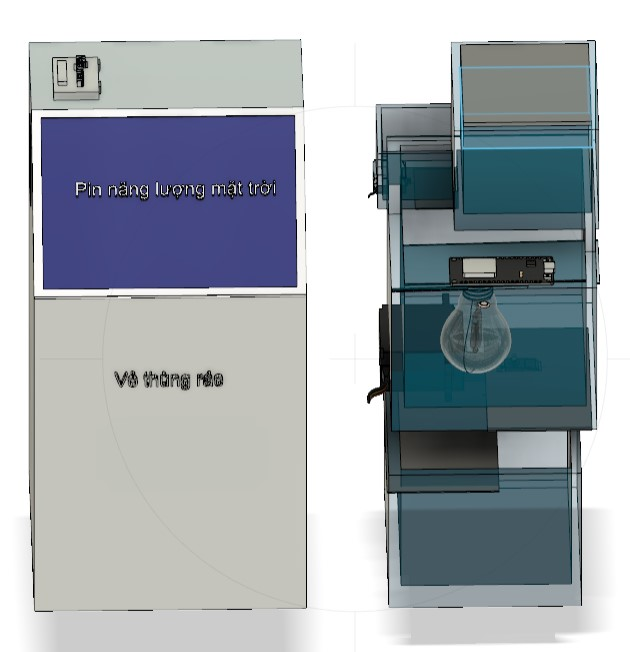
\includegraphics[scale = 1.0]{3D/Outside.jpg}} \\ 
    \item Như hình, mô hình được xây dựng bởi 4 ngăn, gồm: ngăn men, ngăn xay (hay ngăn chứa rác), ngăn ủ, và ngăn thành phẩm. 
    \item Mô hình được phác thảo theo vật liệu trong suốt để có thể thấy được các chi tiết bên trong. Như hình, ta có thể thấy bóng đèn, mạch điện, servo, và một số mảnh vật liệu khác. Ngoài ra, phần vỏ còn cho thấy ta có pin năng lượng mặt trời. \\ \\
    \centerline{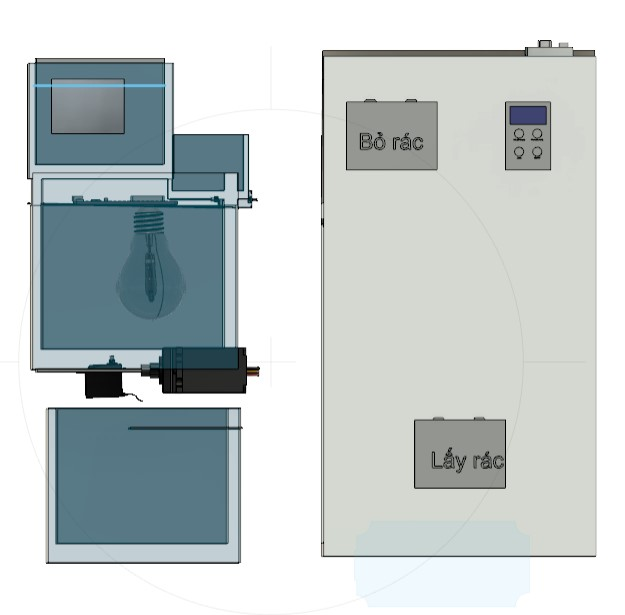
\includegraphics[scale = 1.0]{3D/Behind.jpg}} \\ 
    \item Đây là phác thảo sau lưng mô hình, gồm các nắp đổ rác, ngăn lấy rác, các nút bấm.
    \item Các chi tiết chính của mô hình đều được ghi cụ thể trên từng bộ phận. \\ \\
    \centerline{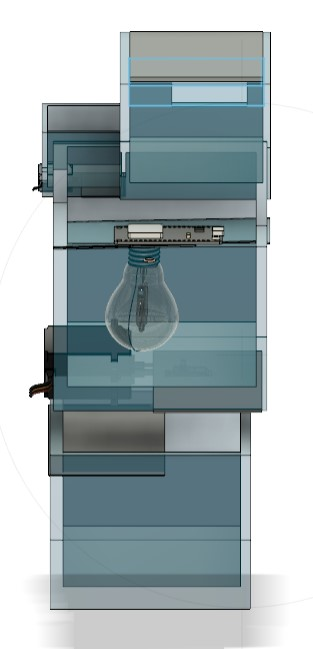
\includegraphics[scale = 1.0]{3D/Inside.jpg}} \\
\end{itemize}

\subsection{Cấu trúc chi tiết}
\begin{itemize}
    \item Trước tiên, ta sẽ tiến hành liệt kê các chi tiết và linh kiện cần thiết cho mô hình.
    \begin{itemize}
        \item Đầu tiên là mạch ESP: \\ \\
        \centerline{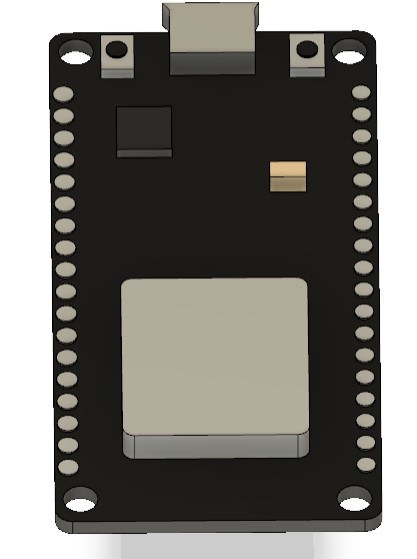
\includegraphics[scale = 0.4]{3D/ESP.jpg}} \\ 
        \centerline{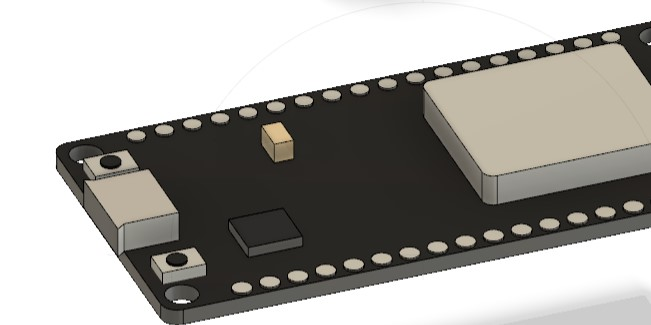
\includegraphics[scale = 0.4]{3D/ESP2.jpg}} \\ 
        \item Bộ phận tiếp theo là Servo: \\ \\
        \centerline{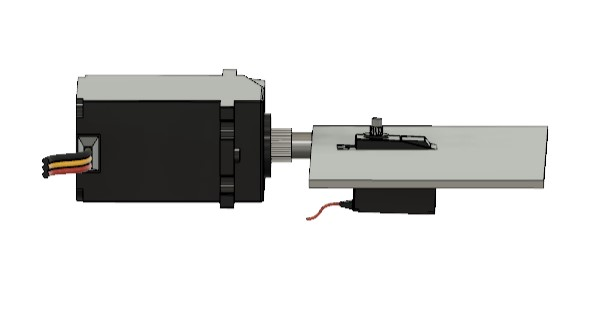
\includegraphics[scale = 0.4]{3D/Servo.jpg}} \\ 
        \centerline{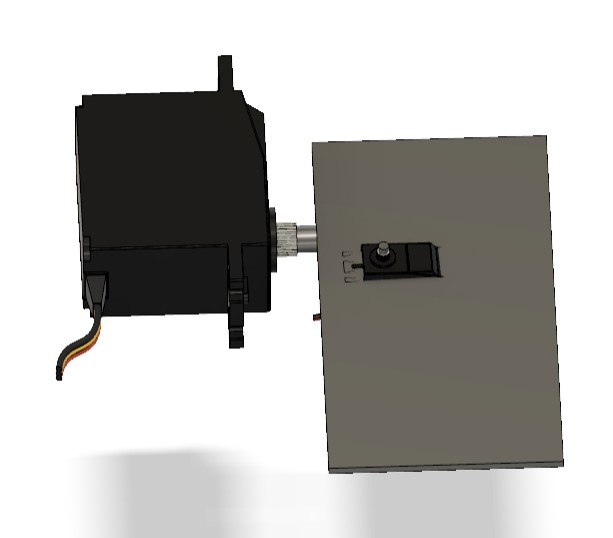
\includegraphics[scale = 0.4]{3D/Servo1.jpg}} \\ 
        \item Bộ phận tiếp theo là Bóng đèn: \\ \\
        \centerline{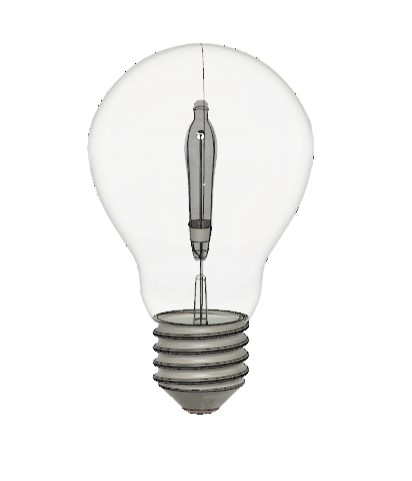
\includegraphics[scale = 0.7]{3D/LightBulb.jpg}} \\ 
        \item Bộ phận tiếp theo là Máy xay rác: \\ \\
        \centerline{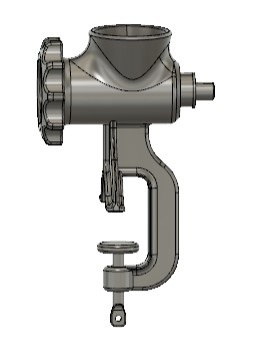
\includegraphics[scale = 0.7]{3D/Grinder.jpg}} \\ 
        \centerline{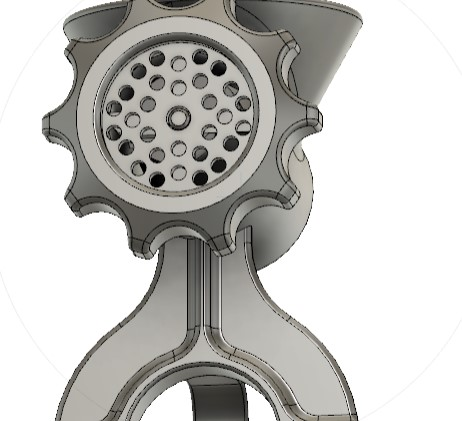
\includegraphics[scale = 0.7]{3D/GrinderFocus.jpg}} \\
        \textnormal{Máy xay rác được lấy ý tưởng từ mô hình máy xay thịt, cấu trúc thực tế cũng sẽ giống cách vận hành này, gồm một lối vào nghiền rác và thải ra vụn rác nhỏ qua các lỗ thoát. Trục máy xoay được gắn với 1 motor để trộn thay vì phải xay bằng tay.}
    \end{itemize}
    \item Và sau đây chúng ta sẽ đến chi tiết các ngăn trong thiết bị. Ngăn đầu tiên là ngăn men, ngăn men có một servo đóng vai trò như một cần gạt đóng mở tự động để nhả số lượng men cần thiết tùy theo khối lượng rác đầu vào: \\ \\ 
    \centerline{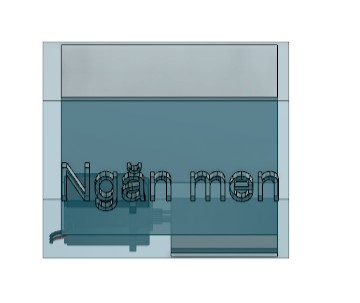
\includegraphics[scale = 0.7]{3D/Menfront.jpg}} \\ \\
    \centerline{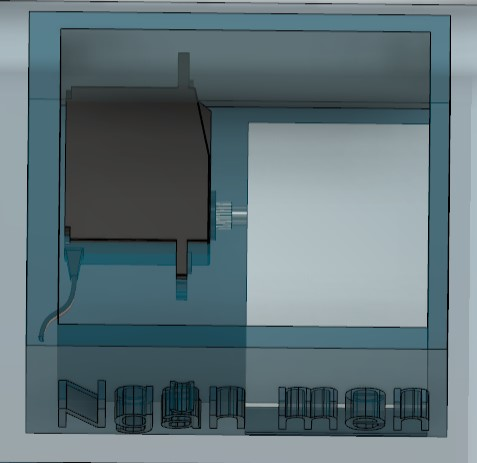
\includegraphics[scale = 0.7]{3D/MenInside.jpg}} \\ 
    \item Ngay bên cạnh ngăn men là ngăn chứa rác (hay ngăn xay). Ngăn này có một máy xay rác dùng để vừa dự trữ rác, vừa xay nhuyễn rác để đẩy rác xuống ngăn ủ, 2 hình bên dưới là ngăn men và ngăn chứa rác. \\ \\
    \centerline{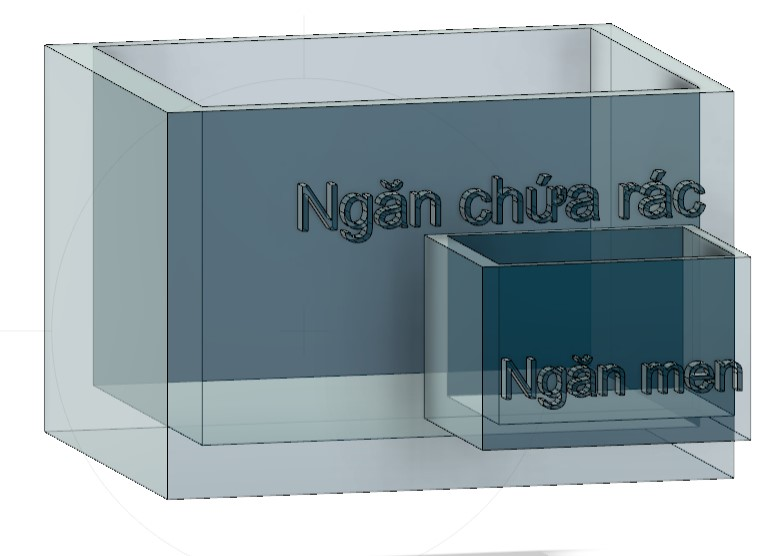
\includegraphics[scale = 0.7]{3D/Rac+Men.jpg}} \\ 
    \centerline{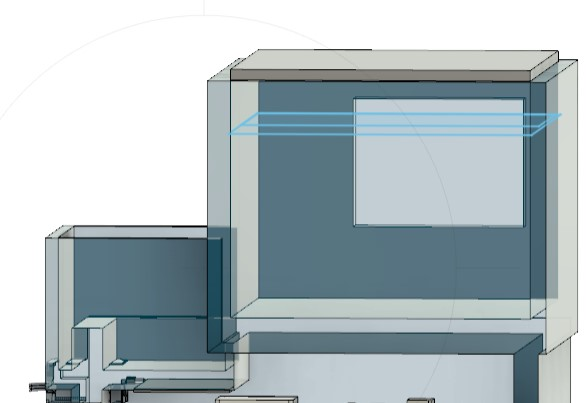
\includegraphics[scale = 0.7]{3D/Rac+MenInResult.jpg}} \\ 
    \item Ngăn chính của thiết bị chính là ngăn ủ phân. Ngăn này có các thiết bị như bóng đèn dây tóc dùng để sưởi ấm và tạo nhiệt độ ủ phân, có servo trộn ngay bên dưới đáy, có servo đóng mở nắp như một cần gạt tự động đến ngăn thành phẩm sau khi phân đã ủ xong. Các hình bên dưới là ngăn ủ từ nhiều góc độ chụp khác nhau.\\ \\
    \centerline{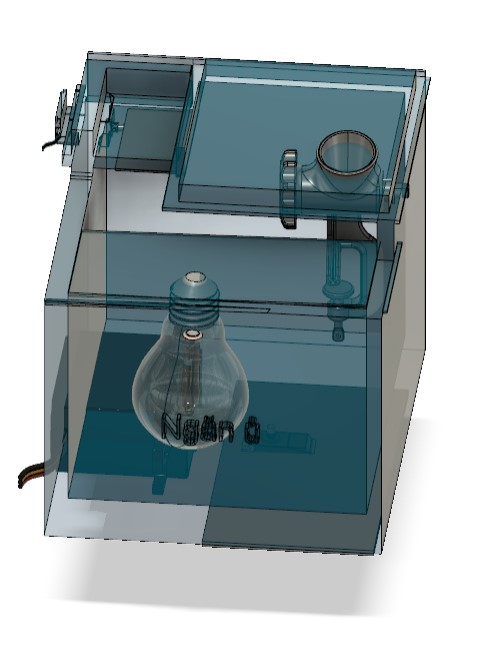
\includegraphics[scale = 0.7]{3D/NganU.jpg}} \\ 
    \centerline{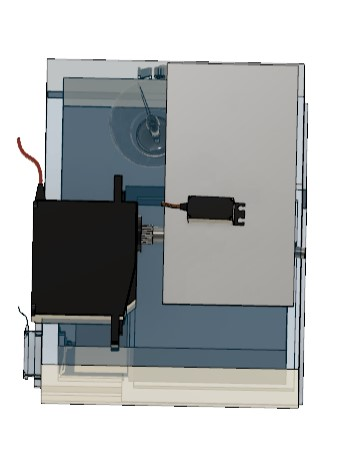
\includegraphics[scale = 0.7]{3D/NganUDown.jpg}} \\
    \centerline{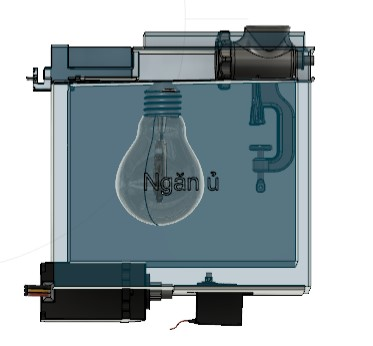
\includegraphics[scale = 0.7]{3D/NganUFront.jpg}} \\ 
    \item Ngăn cuối cùng là ngăn ủ, nhiệm vụ đơn giản là chứa thành phẩm sau khi đã ủ xong cho người dùng lấy. Ngoài ra,   ngăn ủ còn giữ khô và kín phân. \\ \\
    \centerline{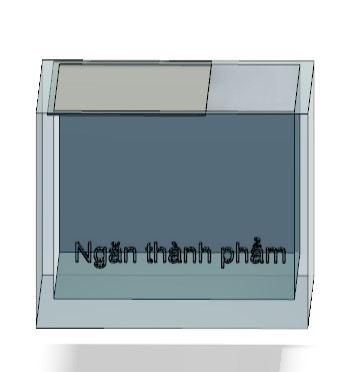
\includegraphics[scale = 0.6]{3D/NganTP.jpg}} \\ \\
    \centerline{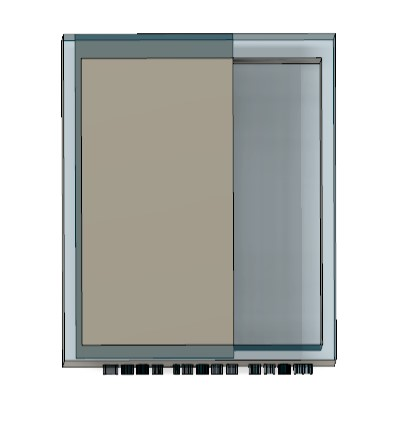
\includegraphics[scale = 0.6]{3D/NganTPUp.jpg}} \\
\end{itemize}
% Huy %
\section{VẬN HÀNH VÀ XỬ LÝ}

\textbf{Thuật toán được triển khai, cài đặt và được kết hợp trên các nền tảng Wokwi cùng với Node-red, ThingSpeak và IFTTT. Đây là tổng quan mô hình thùng ủ phân tự động trên mạch.} \\
\textbf{\href{https://drive.google.com/drive/folders/1SFOhzDiOCOt-AMFM7m-FWzQ3i351csu7?usp=sharing}{Video demo sản phẩm giả lập}} \\
\centerline{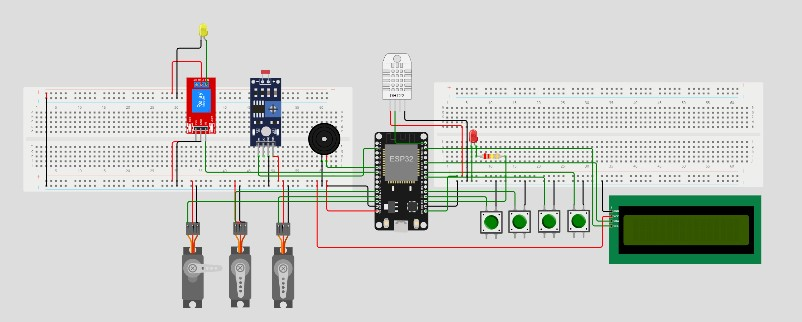
\includegraphics[scale = 1.0]{Wokwi/Board.jpg}} \\
\subsection{Cài đặt, xử lý và xuất thông tin giả lập cho người dùng}
% Huy %
\begin{itemize}
    \item Để người dùng nắm được các thông tin xử lý rác của thiết bị, ta cần truyền các thông số đó lên màn hình LCD.
    Các thông số đó bao gồm: Tiến độ hoàn thành, Thông số nhiệt độ, Thông số độ ẩm, Chế độ rác và Lượng pin của thiết bị.
    \item Để có thể hiện đầy đủ và tường minh các thông tin, ta sẽ áp dụng các hàm của LCD như \textbf{LCD.init()}, \textbf{LCD.backlight()} để tạo độ sáng cho màn hình cũng như là điều chỉnh cursor để các dòng được thể hiện đúng trên màn hình.
    \item Đầu tiên ta sẽ có trạng thái khi LCD hiển thị các mode cho người dùng lựa chọn, có 3 mode là tối đa 2kg, 5kg, 10kg. Nội dung hiển thị như sau: \\ \\
    \centerline{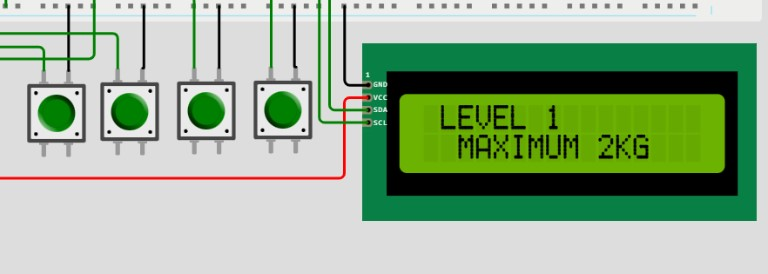
\includegraphics[scale = 0.7]{Wokwi/ModeLCD.jpg}} \\ 
    \item Tiếp theo, khi thiết bị đang hoạt động, người dùng muốn xem đã được bao nhiêu phần trăm thì mode tiến độ sẽ được hỗ trợ trên màn hình. Nội dung cho biết đã hoàn thành được bao nhiêu phần trăm trên tiến độ dự đoán, nội dung như hình sau: \\ \\
    \centerline{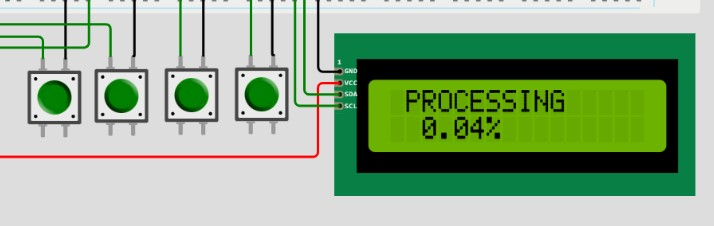
\includegraphics[scale = 0.7]{Wokwi/ProcessLCD.jpg}} \\
    \item Các thông số về nhiệt độ, độ ẩm cũng vô cùng quan trọng, nó cho biết liệu nhiệt độ có đủ ấm và phân bón đã sẵn sàng nhờ độ khô hay chưa. Vì lẽ đó nên màn hình cũng sẽ hiển thị song song 2 thông tin nhiệt độ và độ ẩm. Nội dung chi tiết như các hình sau: \\ \\
    \centerline{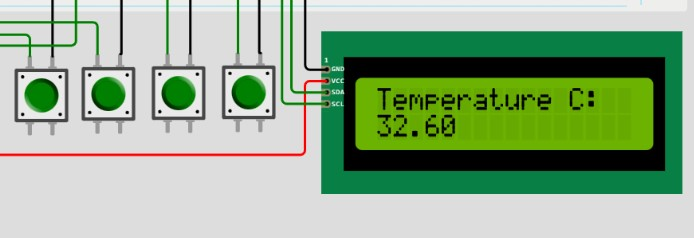
\includegraphics[scale = 0.7]{Wokwi/TempLCD.jpg}} \\ \\
    \centerline{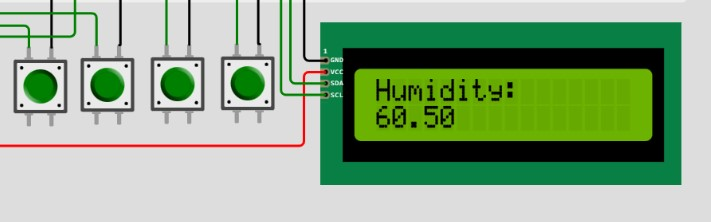
\includegraphics[scale = 0.7]{Wokwi/HmudLCD.jpg}} \\ 
    \item Thông số cuối cùng và cũng không kém phần quan trọng, vì máy được vận hành nhờ nguồn năng lượng mặt trời, nên khi không có ánh sáng, lượng pin của thiết bị sẽ giảm. Chính vì điều đó, người dùng cần theo dõi lượng pin đang có của thùng rác: \\ \\ 
    \centerline{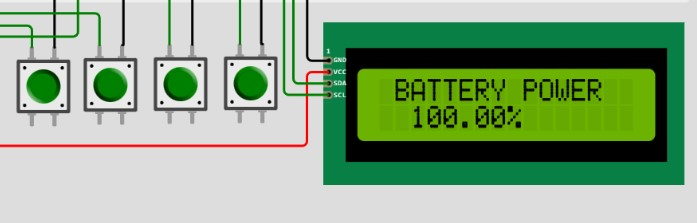
\includegraphics[scale = 0.7]{Wokwi/BatteryLCD.jpg}} \\
\end{itemize}
\subsection{Điều khiển thiết bị giả lập phần cứng}
% Huy %
\begin{itemize}
    \item Để thiết bị có thể chạy đúng theo những gì người dùng yêu cầu, ta cần lập trình sao cho chúng đáp ứng với nhu cầu đó nhưng vẫn nắm được các thông số hoạt động cũng như các bước logic cơ bản của thiết bị mà không làm nghịch lý quá trình diễn ra sự ủ.
    \item Đầu tiên, ta cần lập trình sao cho khi người dùng nhấn vào nút chạy sau khi chọn chế độ bỏ rác thì đèn led sẽ sáng. Đèn led này sáng đồng nghĩa với việc máy đang trong quá trình thực hiện đến khi hoàn thành xong. \\ \\
    \centerline{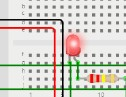
\includegraphics[scale = 1.5]{Wokwi/Led.jpg}} \\
    \item Cùng lúc này, bước tiếp theo người dùng sẽ tiến hành bỏ rác vào thùng, quá trình này dẫn đến việc rác cần được xay nhuyễn. Vì vậy sau khi bật đèn led, ta sẽ kích hoạt máy xay thông qua relay, cũng như bật đèn sưởi để số lượng rác xay nhuyễn được ủ ngay lập tức. \\ \\ 
    \centerline{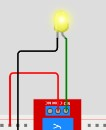
\includegraphics[scale = 1.5]{Wokwi/Light.jpg}} \\ 
    \item Người dùng lựa chọn chế độ rác thì hệ thống sẽ tính toán số lượng men cần thiết cho số lượng rác tương ứng đó. Tính toán xong, hệ thống sẽ nhả men ra tùy theo kích thước rác tương ứng, quy trình nhả men này được thực hiện qua một servo đóng vai trò như một nắp đóng mở tự động. Khối lượng rác nhiều, thì servo mở sẽ lâu hơn và ngược lại.
    \item Trong khi rác đang ủ trong ngăn, sẽ có một servo đóng vai trò như một máy trộn tự động giúp đảo phân bón cho tơi và đều, làm tăng quá trình ủ.
    \item Và sau khi ủ rác xong, một servo thứ 3 sẽ đóng vai trò như một nắp đóng mở tự động đẩy phân từ ngăn ủ xuống ngăn thành phẩm. Và như vậy, chúng ta sẽ có 3 servo với 3 vai trò khác nhau trong việc vận hành xử lý rác thành phân bón. \\ \\
    \centerline{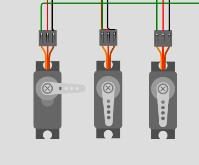
\includegraphics[scale = 1.5]
    {Wokwi/3Servo.jpg}} \\
    \item Tính theo thứ tự từ trái sang phải Servo lần lượt sẽ là: Servo trộn rác, Servo nhả men, Servo ngăn thành phẩm.
\end{itemize}
\subsection{Tính toán số liệu và tiến trình}
% Huy %
\begin{itemize}
    \item Các thông số của thiết bị cần được tính toán gồm có:
    \begin{itemize}
        \item Lượng pin
        \item Tiến độ hoàn thành
        \item Lượng men được nhả
    \end{itemize}
    \item Đầu tiên là lượng pin, để tính lượng pin, thiết bị được hoạt động theo nguyên lý khi có ánh sáng đủ mạnh, pin mặt trời sẽ tiếp nhận và sạc cho ắc quy. 
    \begin{itemize}
        \item Ta đo được độ mạnh yếu, giá trị của ánh sáng dựa vào quang trở, khi quang trở có giá trị cao, ánh sáng sẽ yếu dần. Từ đó ta nhận biết được lượng pin của thiết bị trong tình trạng thiếu ánh sáng.
        \item Cụ thể, ta sẽ lấy ngưỡng quang trở 3000 để nhận biết sự mạnh yếu của ánh sáng, khi quang trở vượt quá 3000, pin sẽ giảm, ngược lại khi quang trở thấp, ánh sáng đủ mạnh để tấm pin mặt trời hấp thụ, pin sẽ tăng.
        \item Ta sẽ dựa vào thời gian quang trở vượt ngưỡng để tính toán sự tiêu hao pin. Cứ mỗi milisecond sẽ chia cho 50000, như vậy sự tiêu hao pin sẽ được giảm theo mỗi milisecond. Trung bình cứ 1 giây khi không có ánh sáng, thiết bị sẽ bị mất khoảng 0,01 đến 0,02 \% pin
        \item Bên cạnh đó, khi ánh sáng đủ mạnh, pin cũng sẽ phục hồi theo một khoảng tính toán mỗi milisecond sẽ chia cho 30000, và như vậy trung bình cứ 1 giây khi ánh sáng đủ mạnh, pin sẽ lại tăng thêm 0,02 đến 0,03 \%.
        \item Khi pin đạt mức 100 \%, thiết bị sẽ không cập nhật thêm lượng pin kể cả khi ánh sáng đủ mạnh.
    \end{itemize}
    \item Thông số tiếp theo, đó là tiến độ hoàn thành. Tiến độ hoàn thành được tính dựa trên sự lựa chọn các mức rác đầu vào từ người dùng.
    \begin{itemize}
        \item Tiến độ được tính tổng quát như sau: \\
        $\textbf{Thời gian ước tính} \div \textbf{Thời gian đã qua kể từ lúc bắt đầu}$
        \item Thời gian bắt đầu được lấy khi người dùng nhấn nút Start trên thiết bị hoặc trên website nhờ hàm \textbf{millis()}.
        \item Cứ mỗi vòng lặp đã qua, một biến \textbf{nowTime} sẽ tự động lấy thời gian hiện. Từ đó ta tính được \textbf{Thời gian đã qua kể từ lúc bắt đầu}. 
        \item Vì trong môi trường giả lập, thời gian ước tính là một con số không quá lớn nhưng cũng tuân thủ logic về sự ủ phân theo các khối lượng rác nhất định. Cụ thể, ở mức rác 1 (tối đa 2 kg), ta có thời gian ước tính là 10000. Mức rác 2 (tối đa 5 kg), thời gian ước tính là 20000. Và cuối cùng mức rác 3 (tối đa 10 kg), thời gian ước tính là 50000.
        \item Từ đó ta sẽ tính toán được thời gian hoàn thành của sản phẩm phân bón và hiển thị cho người dùng thông qua màn hình LCD và website.
    \end{itemize}
    \item Thông số cuối cùng đó là lượng men được nhả, cũng giống như thông số về thời gian tiến độ, lượng men cũng được tính tùy thuộc vào mức rác tương ứng mà người dùng lựa chọn.
    \begin{itemize}
        \item Do không tìm được các thiết bị đo lường khối lượng giả lập, nên ta sẽ quy định sự vận hành của các Servo theo kích thước tương ứng.
        \item Với mức rác 1 (tối đa 2 kg), Servo sẽ tiến hành mở cần gạt ở mức 90 độ cho men rơi xuống với delay là 400. Đây là khoảng thời gian đủ để một mức men nhất định rơi xuống và phù hợp với mức rác.
        \item Với mức rác 2 (tối đa 5 kg), Servo sẽ tiến hành mở cần gạt ở mức 90 độ cho men rơi xuống với delay là 600.
        \item Với mức rác 3 (tối đa 10 kg), Servo sẽ tiến hành mở cần gạt ở mức 90 độ cho men rơi xuống với delay là 800.
    \end{itemize}
\end{itemize}
\subsection{Lập trình kết nối Wifi, MQTT}
% Huy %
\begin{itemize}
    \item Để có thể kết nối được với website, gửi và nhận thông tin từ website, ta cần một giao thức kết nối để đảm bảo hỗ trợ đầy đủ cho các thiết bị vật lý.
    \item MQTT (Message Queuing Telemetry Transport) là giao thức truyền thông điệp (message) theo mô hình publish/subscribe (cung cấp/ thuê bao), được sử dụng cho các thiết bị IoT với băng thông thấp, độ tin cậy cao và khả năng được sử dụng trong mạng lưới không ổn định. Nó dựa trên một Broker (tạm dịch là “Máy chủ môi giới”) “nhẹ” (khá ít xử lý) và được thiết kế có tính mở (tức là không đặc trưng cho ứng dụng cụ thể nào), đơn giản và dễ cài đặt.
    \item Thiết bị kết nối vào mạng WIFI được gọi là station (trạm). Việc kết nối vào mạng Wifi được hỗ trợ bởi một access point (AP), một AP có chức năng như một hub nhưng dùng cho nhiều station. Một access point thông thường được kết nối vào một mạng dây để phát WIFI (tức là chuyển từ mạng dây sang WIFI). Do đó access point luôn được tích hợp vào router. Mỗi access point được nhận biết bằng một SSID (Service Set IDentifier), SSID cũng là tên của mạng hiển thị khi ta kết nối vào WIFI.
    \item Thư viện \textbf{ESP8266WiFi.h} có hỗ trợ các câu lệnh để module thưc hiện việc kết nối vào WIFI (làm chức năng của station).
    \item Để có thể kết nối Wifi cũng như sử dụng thông qua giao thức MQTT, ta cần cài đặt các thư viện sau:
    \begin{lstlisting}
        #include <WiFiClient.h>
        #include <ESP8266WiFi.h>
        #include <PubSubClient.h>\end{lstlisting}
    \item Sau đó, ta tiến hành cài đặt các hàm cần thiết như \textbf{wifiConnect()}, \textbf{mqttConnect}, \textbf{sendRequest}, \textbf{callBack} để có thể kết nối giữa Wokwi và Node-red.
\end{itemize}
\subsection{Nhận thông tin từ Website}
% Huy %
\begin{itemize}
    \item Hàm \textbf{callBack()} được xây dựng để hỗ trợ nhận thông tin từ Website về Wokwi.
    \item Cụ thể, website sẽ trả về 1 số dạng chuỗi tương ứng với từng chức năng.
    \begin{itemize}
        \item Nếu số đó là 0 - 1 - 2, đó chính là 3 mức rác của người dùng lựa chọn trên website, tương ứng với ít rác, rác vừa, nhiều rác và cũng là tín hiệu Start.
        \item Nếu đó là số 4, nghĩa là người dùng đang yêu cầu Pause hệ thống trên website và ta cần xử lý dừng trong đoạn mã lâp trình.
    \end{itemize}
\end{itemize}
\subsection{Lấy thời gian thực trên mạch}
% Chương %
\begin{itemize}
    \item Thiết lập một đối tượng \textbf{NTPClient} có khả năng liên kết với máy chủ NTP tại \textbf{"vn.pool.ntp.org"}, sẵn sàng để cập nhật thời gian.
    \item \textbf{timeClient.forceUpdate()}: Đây là một phương thức gọi để cập nhật dữ liệu thời gian từ máy chủ NTP thông qua các thư viện sau:
    \begin{lstlisting}
        #include <NTPClient.h>
        #include <WiFiUdp.h>\end{lstlisting}    
    \item \textbf{strftime(startDate, sizeof(startDate), "\%Y-\%m-\%d", timeinfo)}: Đoạn mã này sử dụng hàm \textbf{strftime} để định dạng ngày hiện tại thành chuỗi có định dạng "Năm/Tháng/Ngày" và lưu vào biến \textbf{startDate}.
    \item \textbf{int daysToAdd = DateExpect + mode}: Biến \textbf{daysToAdd} là tổng của hai biến \textbf{dateExpect} và \textbf{mode}.
    \item \textbf{timeinfo->tm\_mday += daysToAdd}: Thêm số ngày từ biến \textbf{daysToAdd} vào ngày hiện tại.
    \item \textbf{time\_t newTimestamp = mktime(timeinfo)}: Chuyển đổi cấu trúc \textbf{struct tm} đã được thay đổi thành một timestamp mới bằng cách sử dụng hàm \textbf{mktime}.
    \item Sau đó, cập nhật \textbf{timeinfo} để thể hiện ngày mới tính toán và sử dụng hàm \textbf{strftime} để định dạng ngày kết thúc, sau đó in ra ngày kết thúc.
\end{itemize}
\subsection{Đẩy thông tin lên website (dạng JSON)}
% Chương %
\begin{itemize}
    \item Sử dụng mqtt request để đẩy thông tin lên node-red thông qua mqttClient.publish() và thư viện.
    \begin{lstlisting}
        #include <ArduinoJson.h>\end{lstlisting}
    \item Trong mã nguồn sử dụng hàm datapush() nhiệm vụ chính của hàm này là đóng gói các thông tin liên quan trong quá trình xử lý vào một đối tượng JSON và sau đó gửi đối tượng JSON này thông qua giao thức MQTT.
    \item \textbf{StaticJsonDocument<200> jsonDoc}: Đây là việc tạo một đối tượng JSON tĩnh (không cần phải cấp phát động) với dung lượng tối đa là 200 bytes. Đối tượng JSON này sẽ được sử dụng để đóng gói thông tin.
    \item Đóng gói JSON gồm các thuộc tính:
        \begin{lstlisting}
var jsonDoc = {
    "temperature": 25, // Nhiet do trong thung u
    "humidity": 60,    // Do am trong thu u
    "start_time": "2023-08-1", // Ngay bat dau
    "completion_time": "2023-08-18", // Ngay du doan ket thuc
    "processing": 55, // Uoc luong muc do hoan thanh
    "message": "Processing is underway.", // Tin nhan
    "emergency": "Nothing.", // Tin nhan truong hop khan cap
    "battery": 80 // Phan tram pin con lai
  };\end{lstlisting}
    \item \textbf{serializeJson(jsonDoc, jsonString)}: Dòng này chuyển đối tượng JSON (jsonDoc) thành một chuỗi JSON (jsonString) bằng cách sử dụng hàm serializeJson.
    \item \textbf{mqttClient.publish("smartbin/data", jsonString.c\_str())}: Cuối cùng, đoạn mã này sử dụng đối tượng MQTT (mqttClient) để gửi chuỗi JSON (jsonString) thông qua kênh MQTT có tên "smartbin/data".
\end{itemize}
\subsection{Gửi thông báo qua điện thoại}
% Chương %
\begin{itemize}
    \item Gửi thông báo khẩn cấp qua điện thoại thông qua app \textbf{ifttt}
    \item Sử dụng chức năng \textbf{Webhook} và \textbf{Notification} để gửi tín hiệu http request cho ifttt và sau đó Notification thông báo về nhưng trường hợp khẩn cấp về cho điện thoại \\ \\
    \centerline{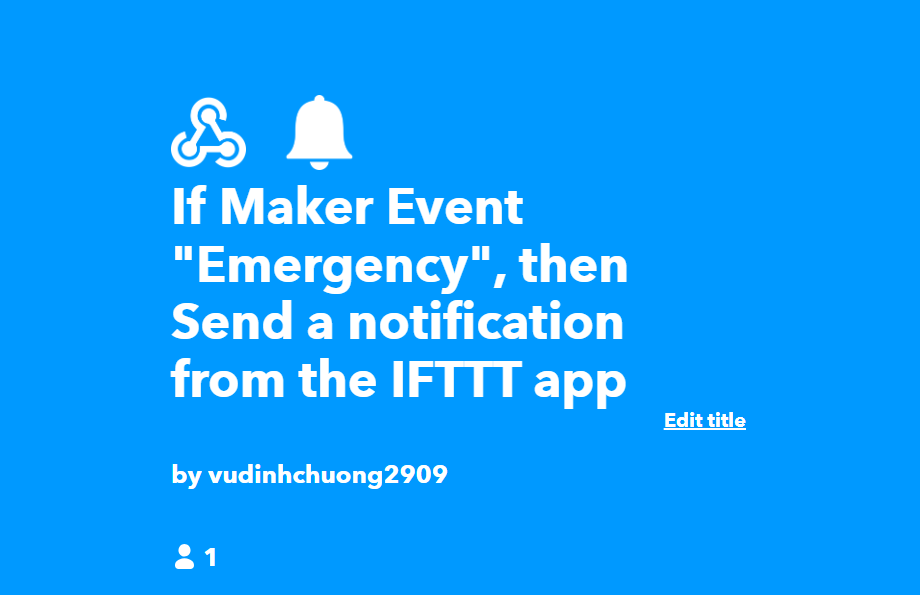
\includegraphics[scale = 0.5]{ifttt/ifttt1.png}} \\ \\
    \centerline{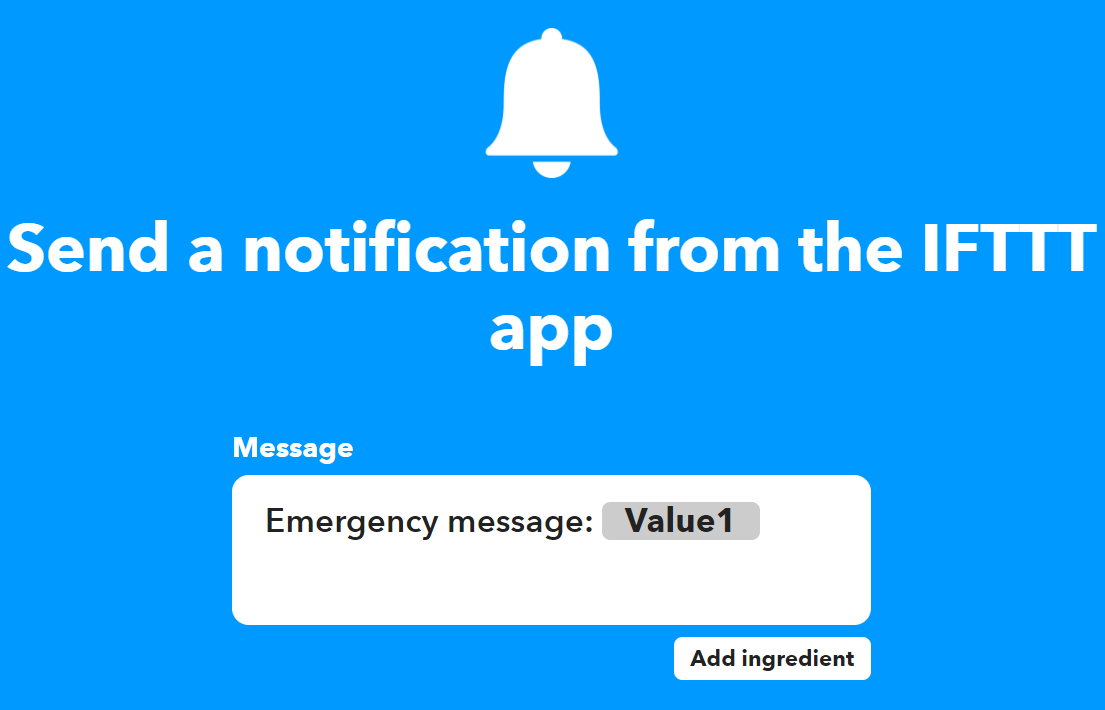
\includegraphics[scale = 0.415]{ifttt/ifttt2.png}} \\ 
    \item Sau khi đã lấy được đường dẫn http. Trong mã nguồn sử dụng http request phương pháp GET để chuyển dữ liệu.
    \item Connect \textbf{port = 80} với \textbf{host = "maker.ifttt.com"} và \textbf{request = "/trigger/emergency/with/key/bjIGHAgSupsGTVdiaLuzjnpRgh9Pz3 \_-DibMKO0io52?}\textbf{value1 = Low\_Battery"} với trường hợp khẩn cấp là Low Battery.
    \item Khi trường hợp khẩn cấp sảy ra sẽ gửi về cho người dùng với thông báo \textbf{Emergency message: {{Value1}}} với \textbf{Value1 = Low\_Battery}. \\ \\
    \centerline{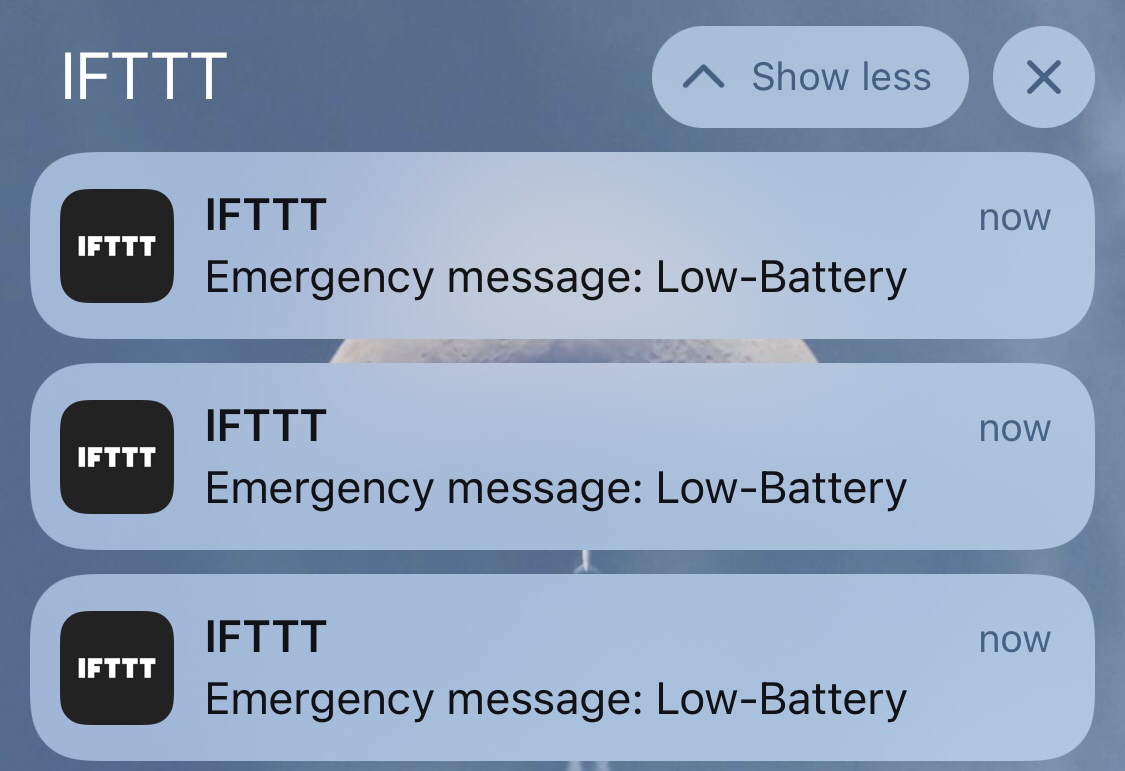
\includegraphics[scale = 0.35]{ifttt/ifttt3.png}} \\ 
\end{itemize}
\subsection{Gửi thông tin từ mạch lên Cloud}
% Chương %
\begin{itemize}
    \item Tương tự như việc gửi thông báo qua điện thoại, ta dùng HTTP request gửi thông  tin lên Cloud-Thinkspeak.\\ \\
    \centerline{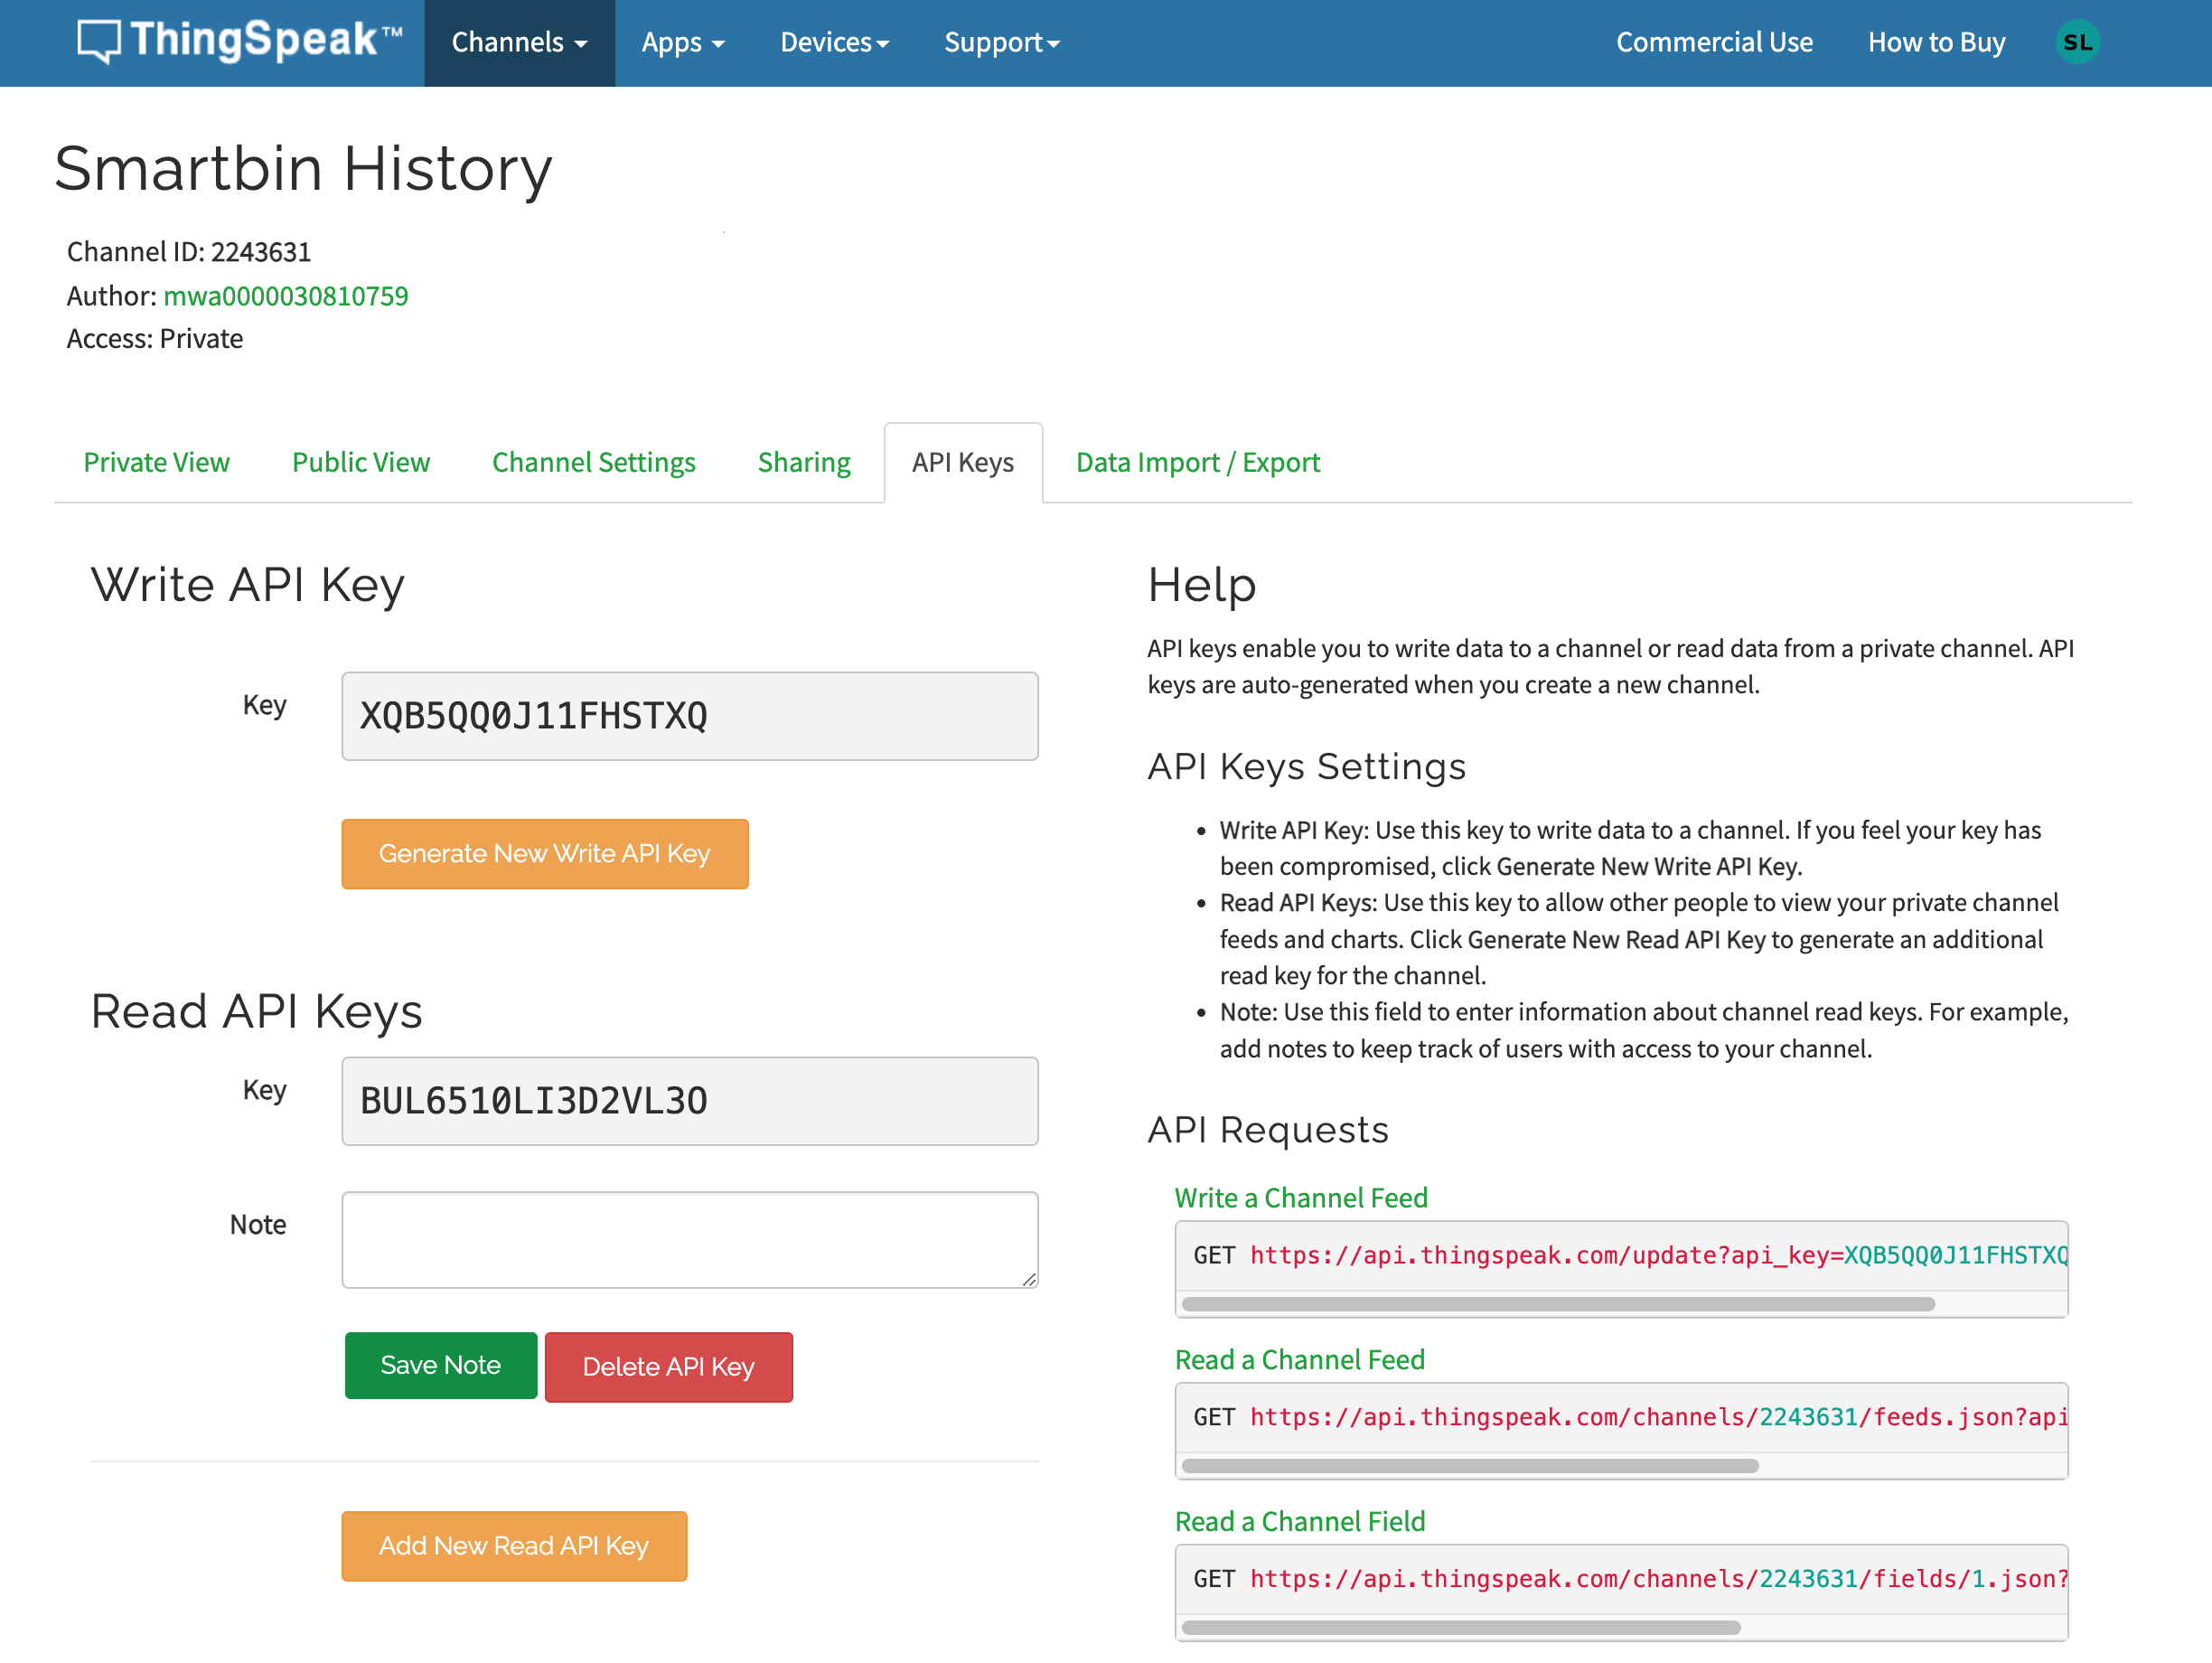
\includegraphics[scale = 0.3]{cloud/cloud1.png}} \\ 
    \item \textbf{host = "api.thingspeak.com"} và với \textbf{request = "/update?api \_key=XQB5QQ0J11 FHSTXQ\&field1=\&field2=\&field3=\&field4="} với tương ứng các giá trị của các field là ngày bắt đầu, ngày kết thúc và tin nhắn khẩn cấp khi máy hoạt động. \\ \\
    \centerline{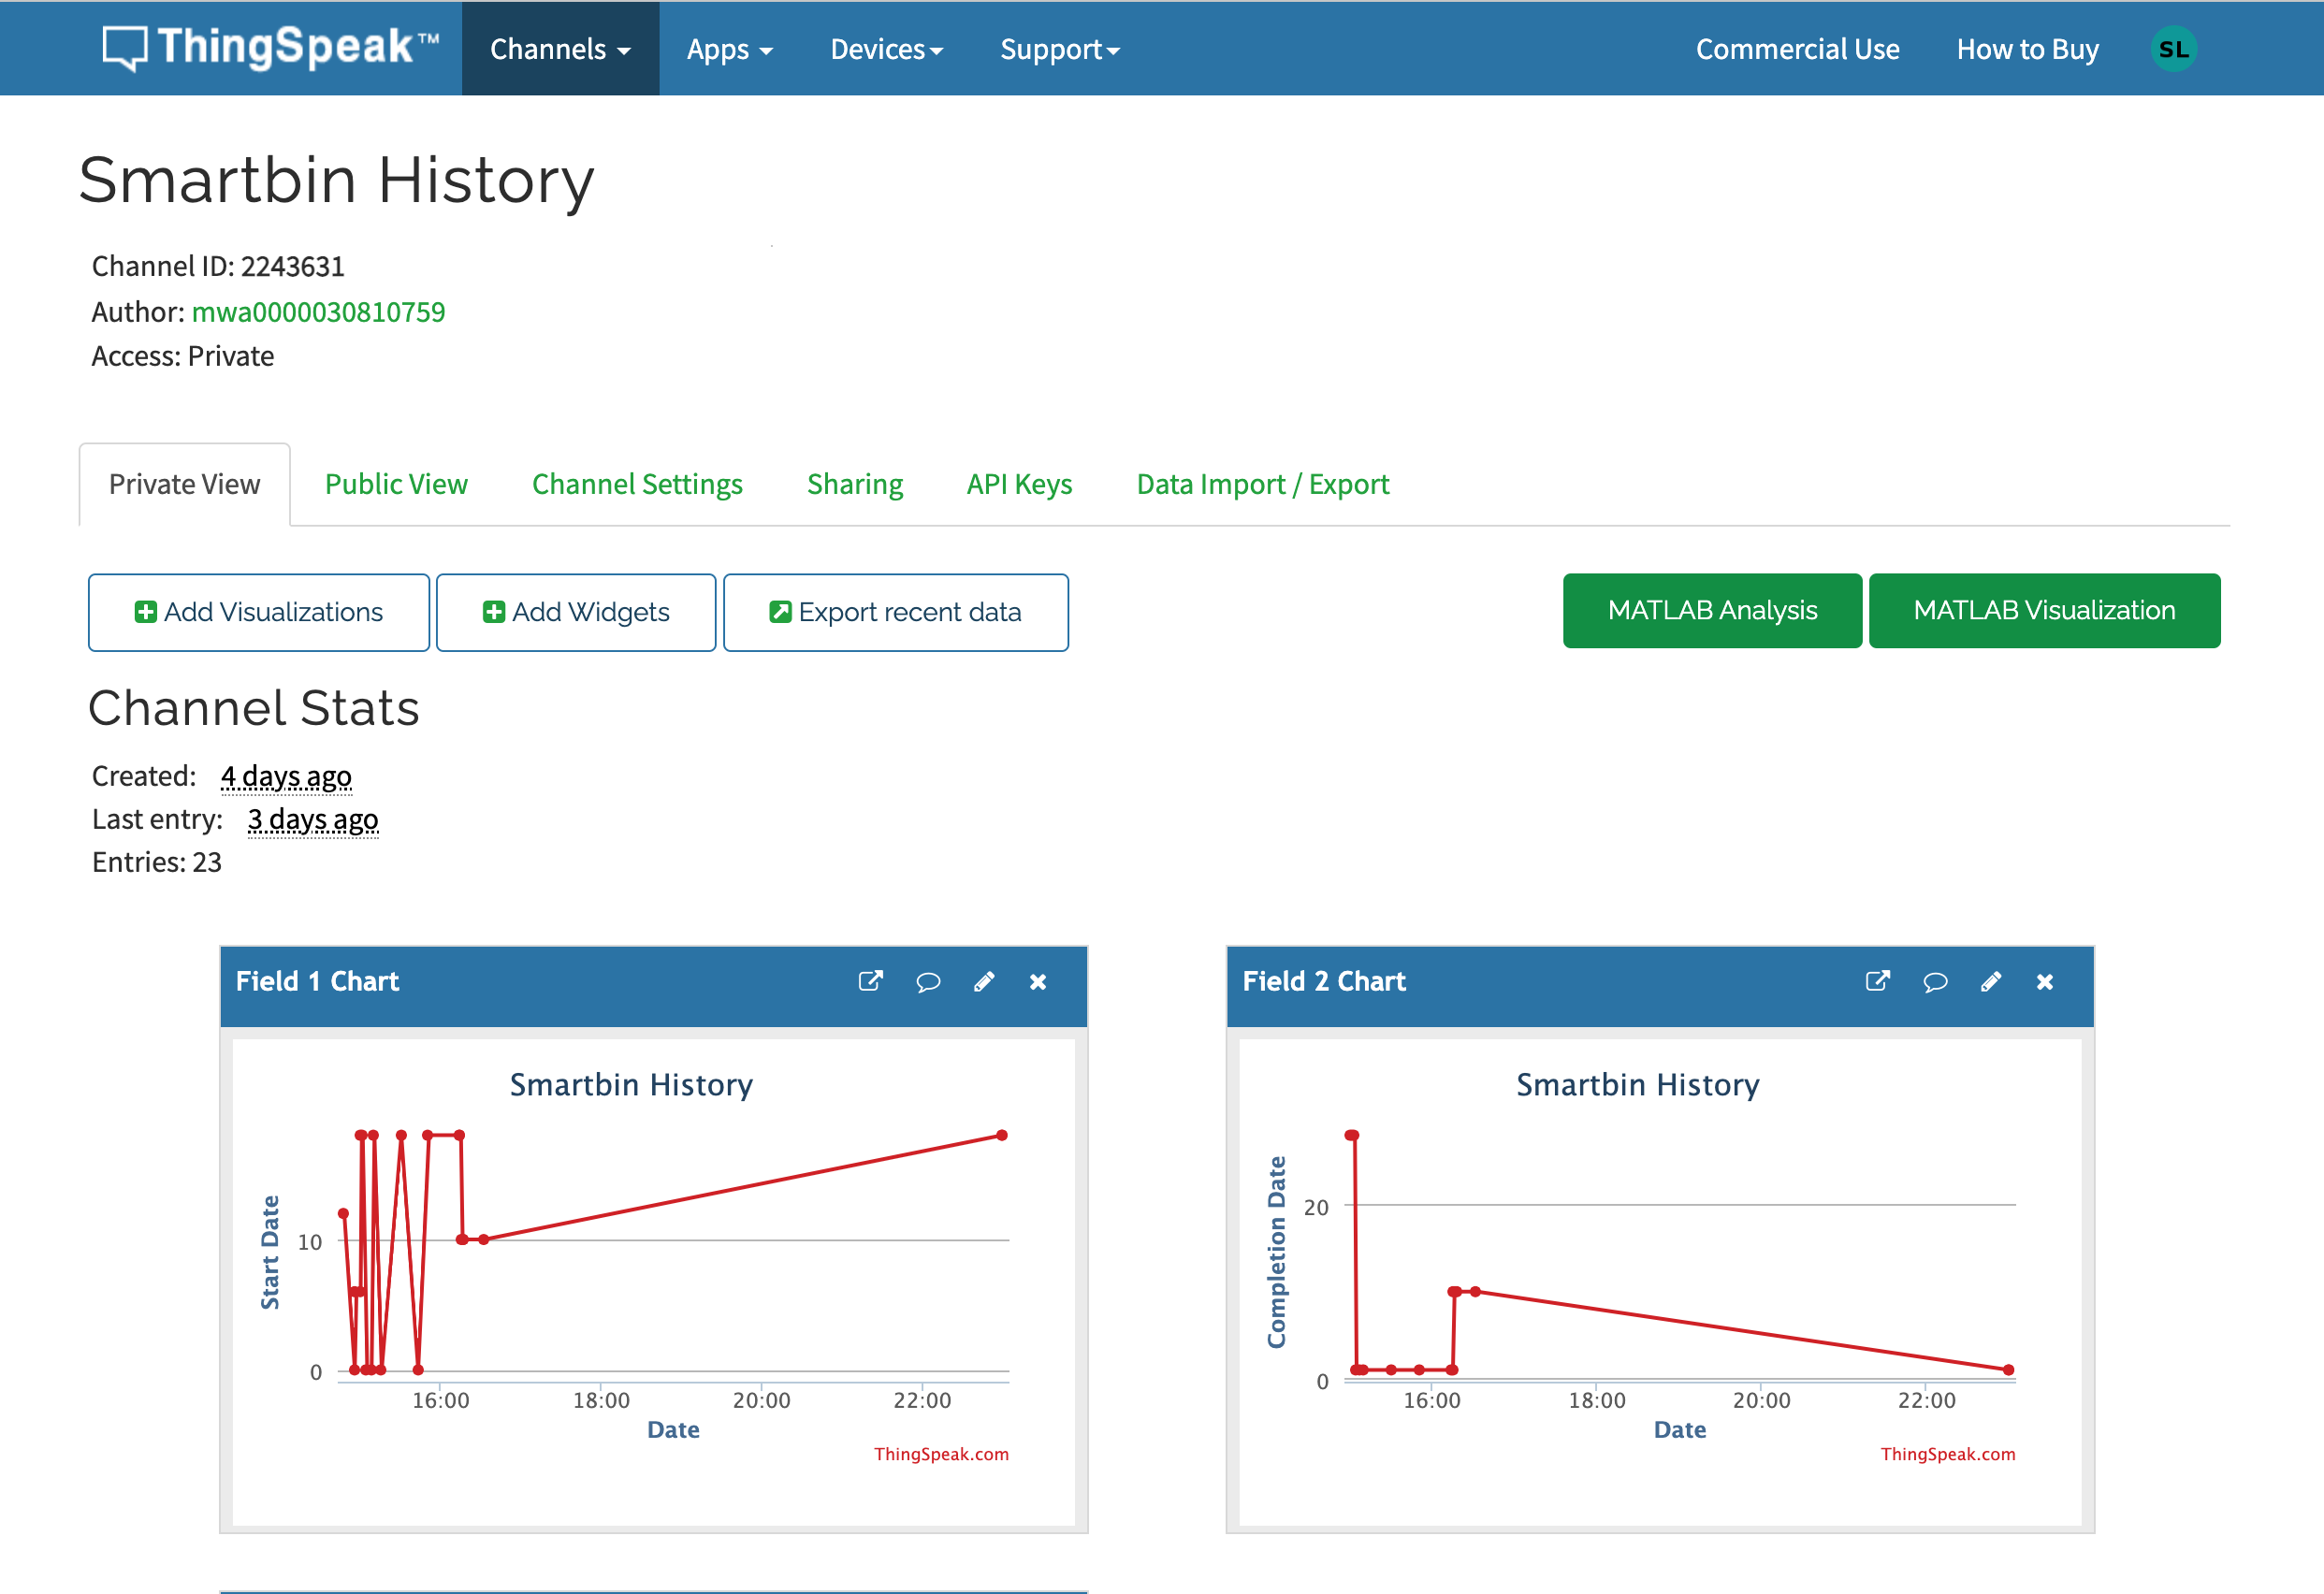
\includegraphics[scale = 0.3]{cloud/cloud2.png}} \\ 
\end{itemize}
\subsection{Xử lý tính logic của mạch và các tình huống khẩn cấp}
% Chương %
\begin{itemize}
    \item  Dưới đây là sơ đồ truyền và nhận dữ liệu giữa các đối tượng trong hệ thống IoT \\ \\
\end{itemize}
\centerline{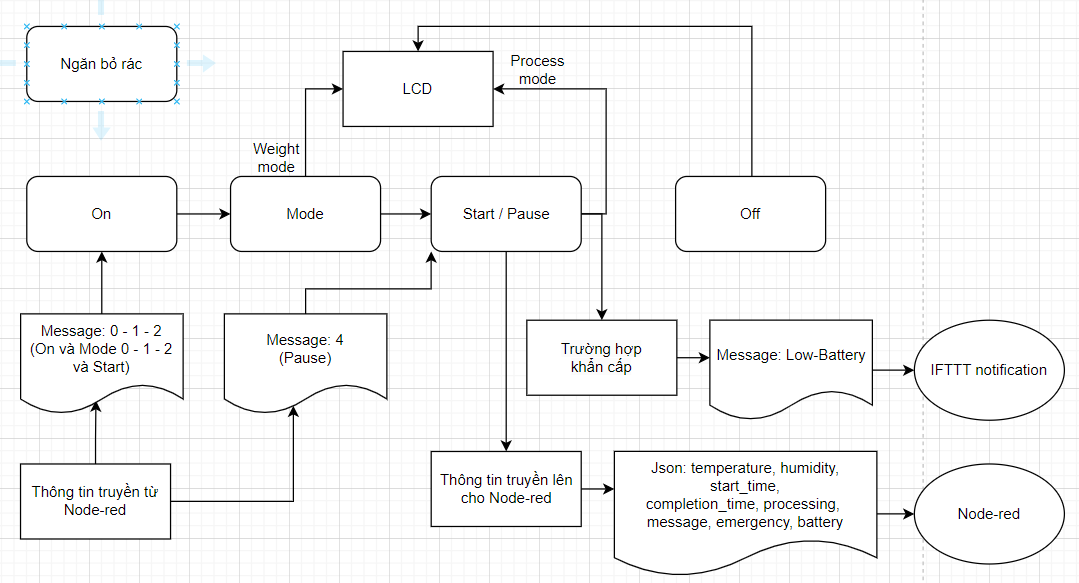
\includegraphics[scale = 0.5]{chart/chart1.png}} \\
\begin{itemize}
    \item Sử nút On để khởi động máy, chọn Mode để thể chọn mức độ nặng của rác bỏ vào để máy xả bộ men phù hợp. Sau đó nhấn nút Start để khởi động.
    \begin{itemize}
        \item Khi bắt đầu khời động máy sẽ lấy dữ liệu sau đó gửi lên cho node-red đồng thời cũng thể hiện lên trên trong LCD. Khi pin yếu Trường hợp khẩn cấp sẽ gửi thông báo về điện thoại thông qua app IFTTT. 
        \item Có thể nhấn nút Mode để chuyển sang các thông báo khác như Nhiệt độ và độ ẩm, Pin, Phần trăm xử lý.
        \item Có thể nhấn lại nút Start để Pause thì sẽ hiển thị \textbf{PAUSE} lên LCD đến khi nhấn lại nút Start lần nữa.
    \end{itemize}
    \item Có thể thực hiện bật mở máy thông qua website Node-red bằng cách chọn Weight và Start trên web sau đó máy sẽ mở lên và hoạt động như trên. Có thể sử dụng Pause trên web để tạm dừng máy.
    \item Bấm nút Off để tất máy và lấy sản phầm ở ngăn thành phẩm
\end{itemize}
\centerline{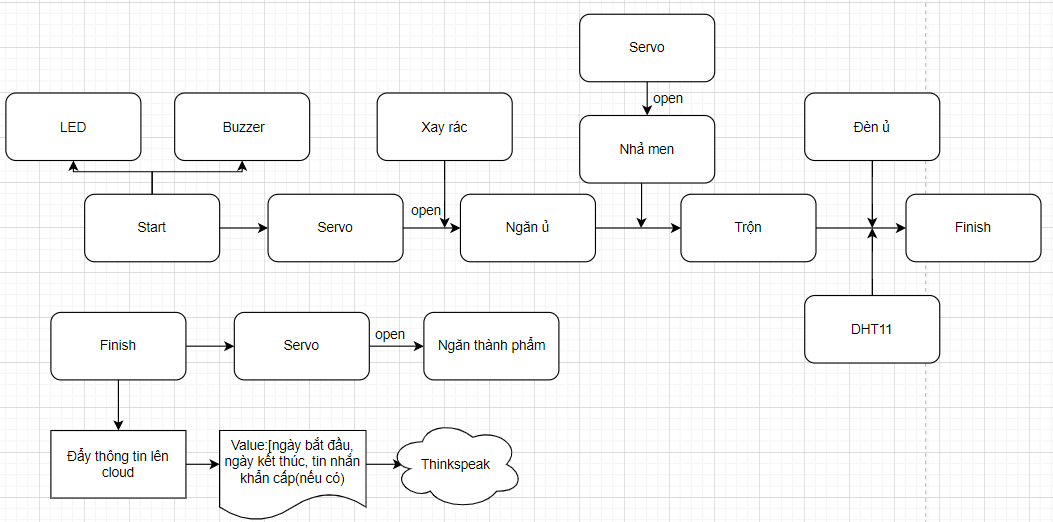
\includegraphics[scale = 0.5]{chart/chart2.png}} \\
\begin{itemize}
    \item Sau khi máy bắt đầu chạy thì LED sáng và Buzzer kêu lên để báo hiệu bắt đầu quá trình ủ. Men sẽ được nhả xuống đồng thời máy xay sẽ xay nhuyễn rác ra. Sau đó sẽ trộn hỗn hợp rác với men và nhiệt độ từ đèn ủ để dần dần thành phân bón. Cảm biến nhiệt độ và độ ẩm sẽ thông báo nhiệt độ và độ ẩm trong thùng ủ.
    \item Khi hoàn thành thì phân bón sẽ trả ra ở ngăn thành phẩm, LED sẽ tắt và Buzzer sẽ báo hiệu tín hiệu kết thúc. Đồng thời sẽ gửi thông tin ngày bắt đầu, ngày kết thúc, tín hiệu khẩn cấp (nếu có) vào Cloud-Thinkspeak để lưu lại.
\end{itemize}
\section{Điều khiển và thông tin từ Website}
\subsection{Hình ảnh giao diện website} 
% Chương %
\newpage
\begin{figure}[!h]
        \centering
        \begin{subfigure}{\textwidth}
            \centering
            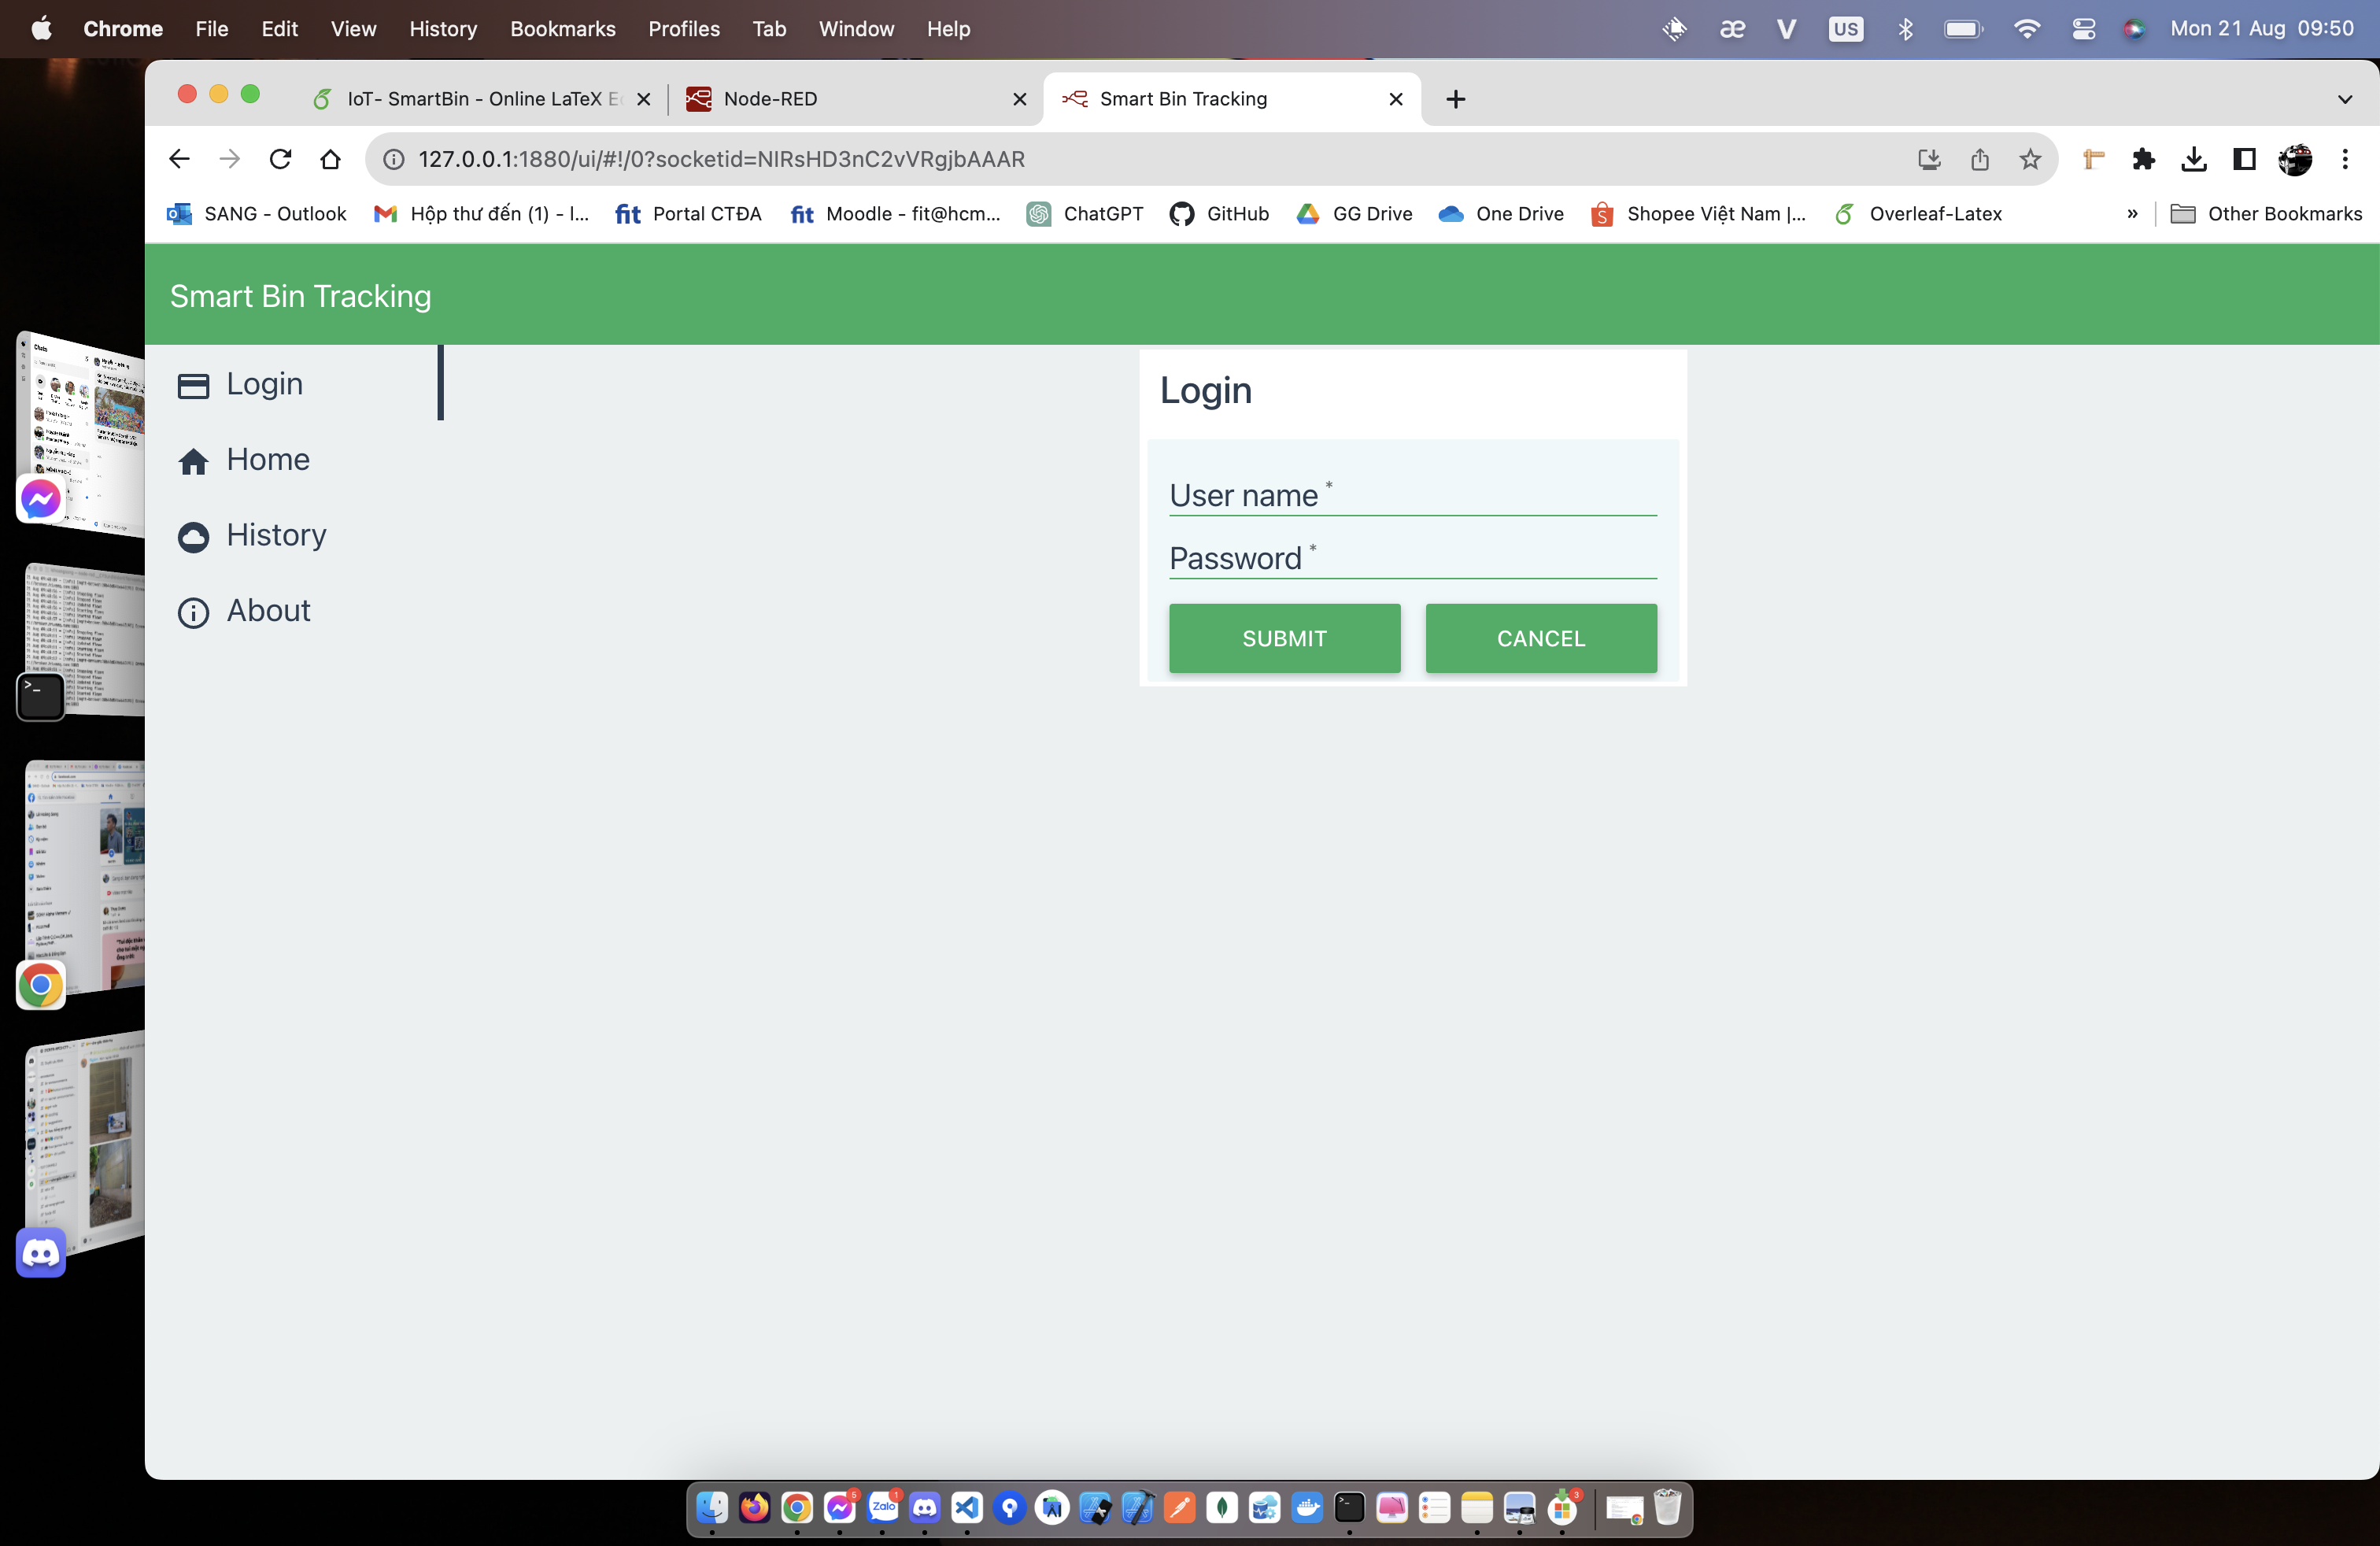
\includegraphics[width=0.9\linewidth]{Node/node-red-login.png}
            \caption{Hình ảnh minh họa Node-Red tab Login.}
        \end{subfigure}
        \begin{subfigure}{\textwidth}
            \centering
            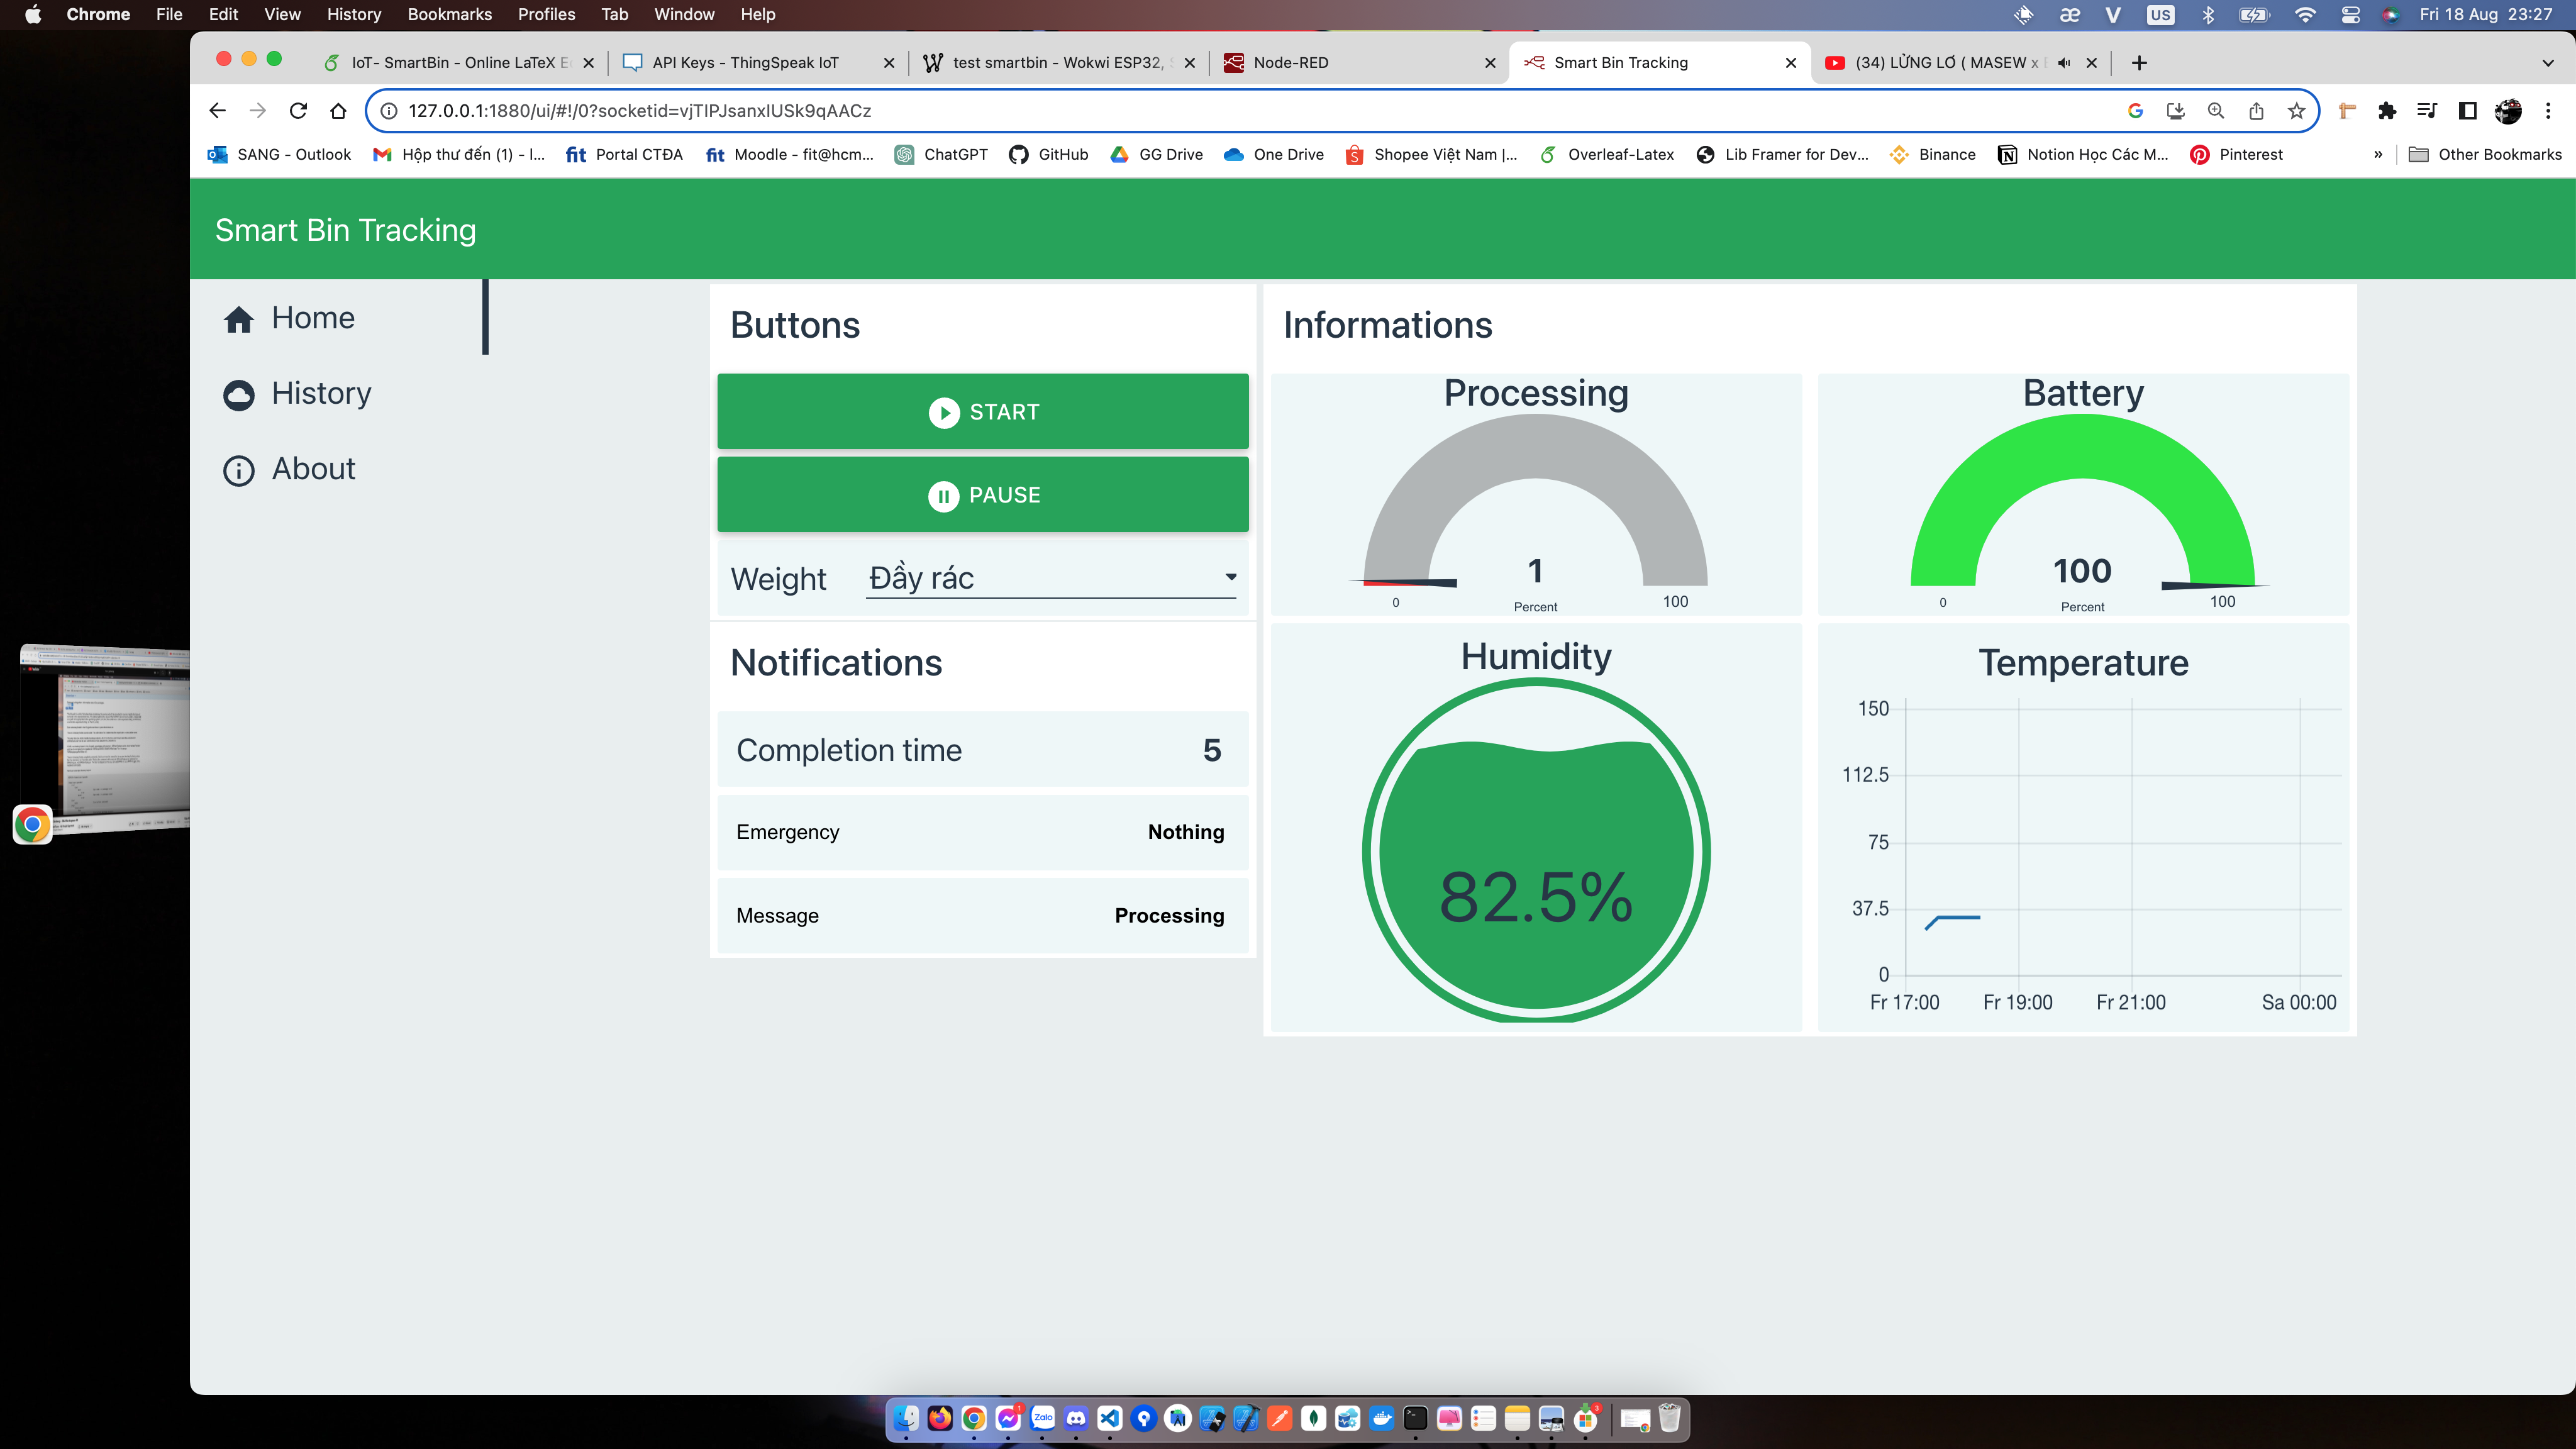
\includegraphics[width=0.9\linewidth]{Node/node-red-home.png}
            \caption{Hình ảnh minh họa Node-Red tab Home.}
        \end{subfigure}
\end{figure}
\pagebreak
\begin{figure}[!h]
        \centering
        \begin{subfigure}{\textwidth}
            \centering
            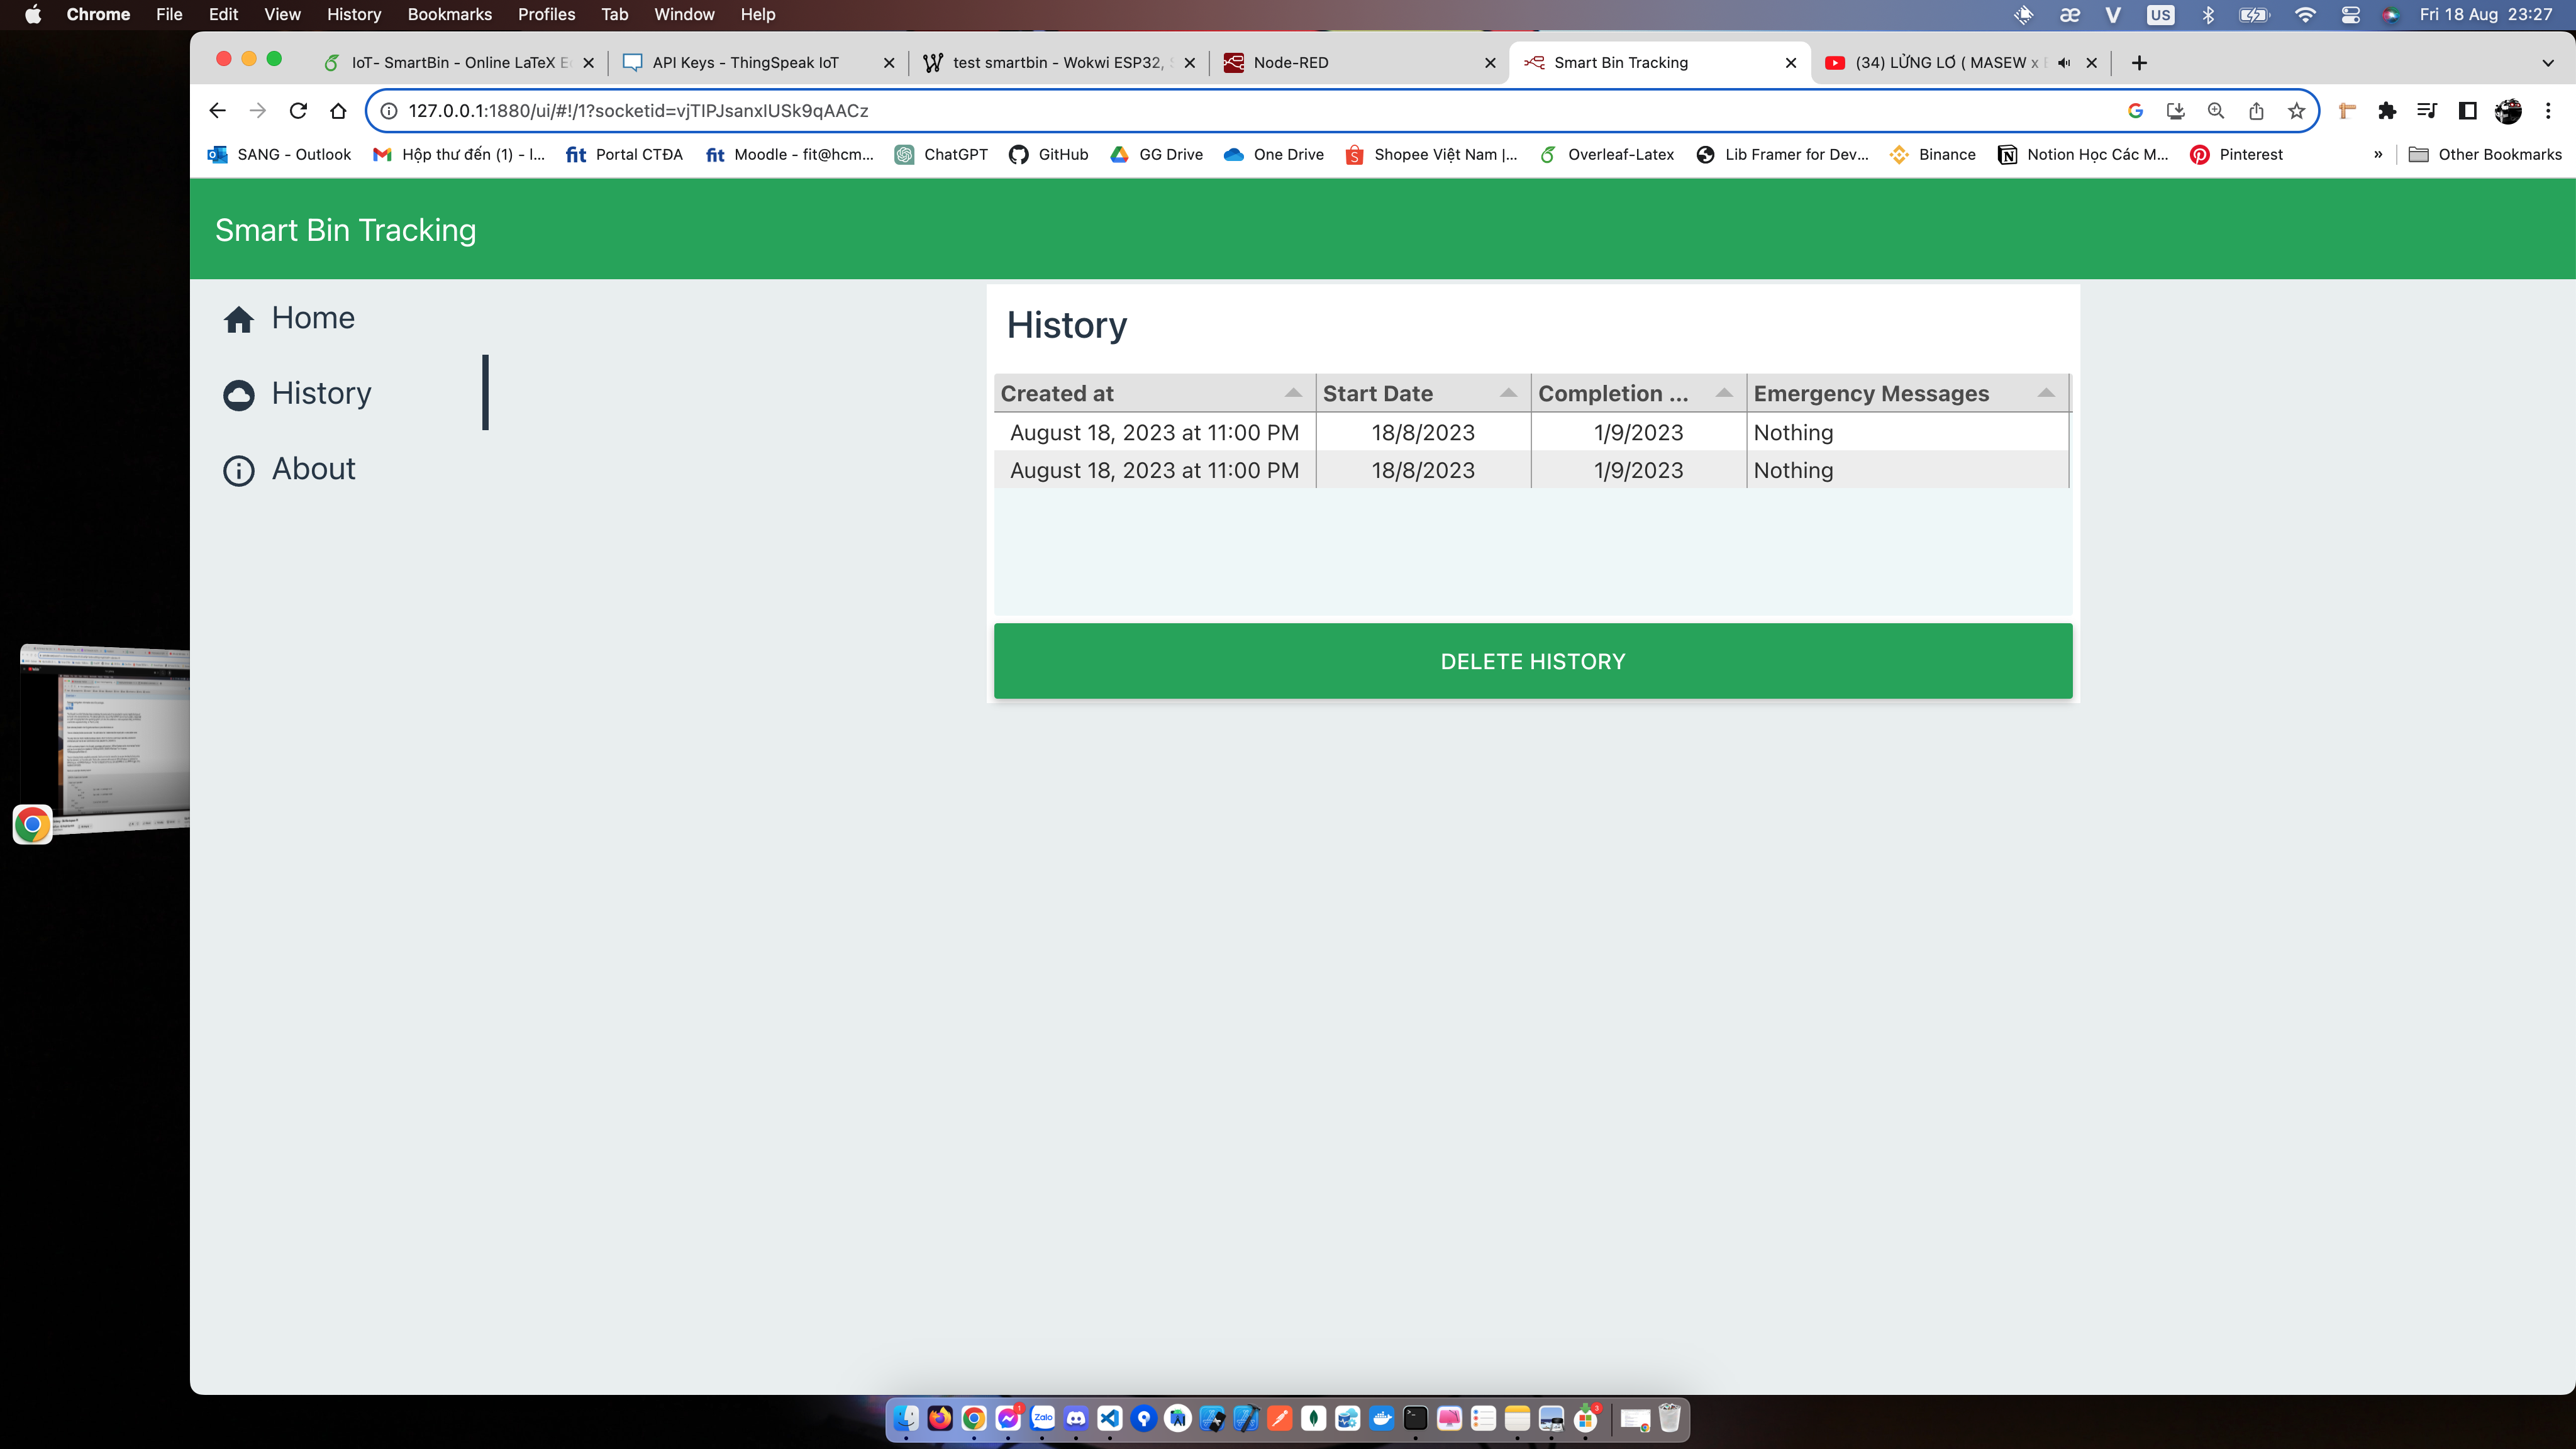
\includegraphics[width=0.9\linewidth]{Node/node-red-history.png}
            \caption{Hình ảnh minh họa Node-Red tab History.}
        \end{subfigure}
        \begin{subfigure}{\textwidth}
            \centering
            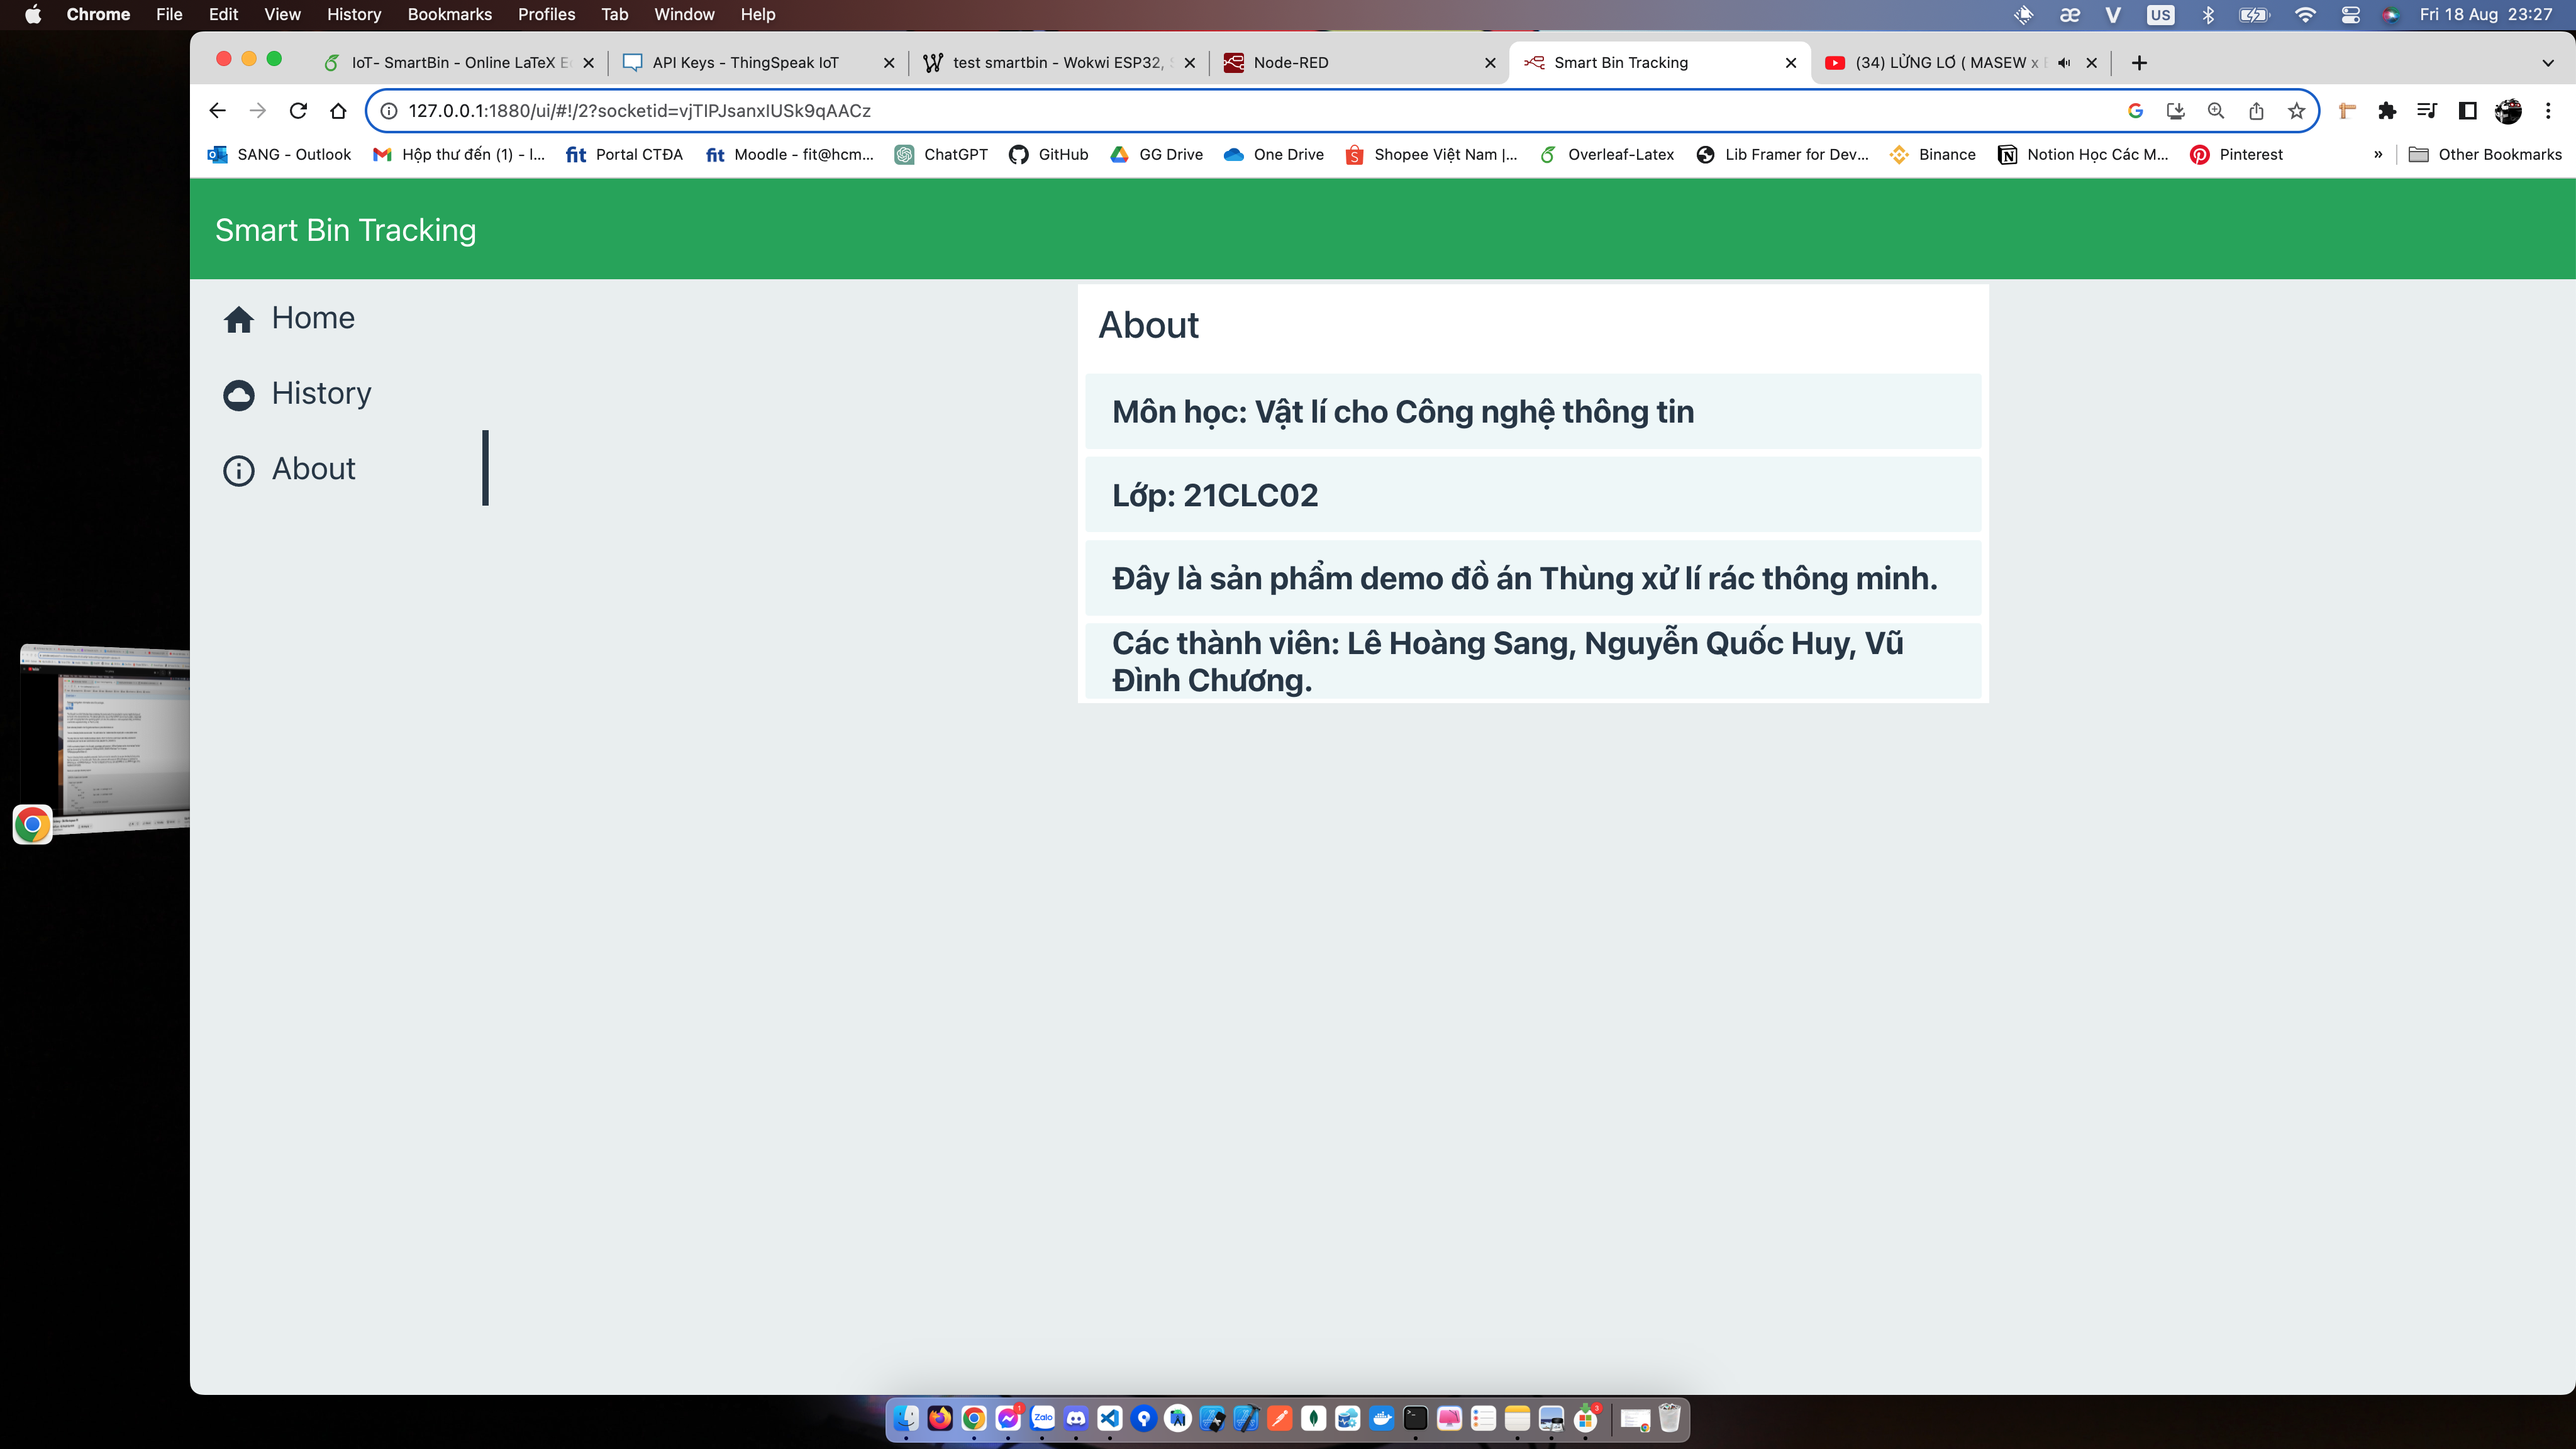
\includegraphics[width=0.9\linewidth]{Node/node-red-about.png}
            \caption{Hình ảnh minh họa Node-Red tab About.}
        \end{subfigure}
\end{figure}
\newpage
\subsection{Hình ảnh cấu trúc nodes}
\begin{figure}[!h]
        \centering
        \begin{subfigure}{\textwidth}
            \centering
            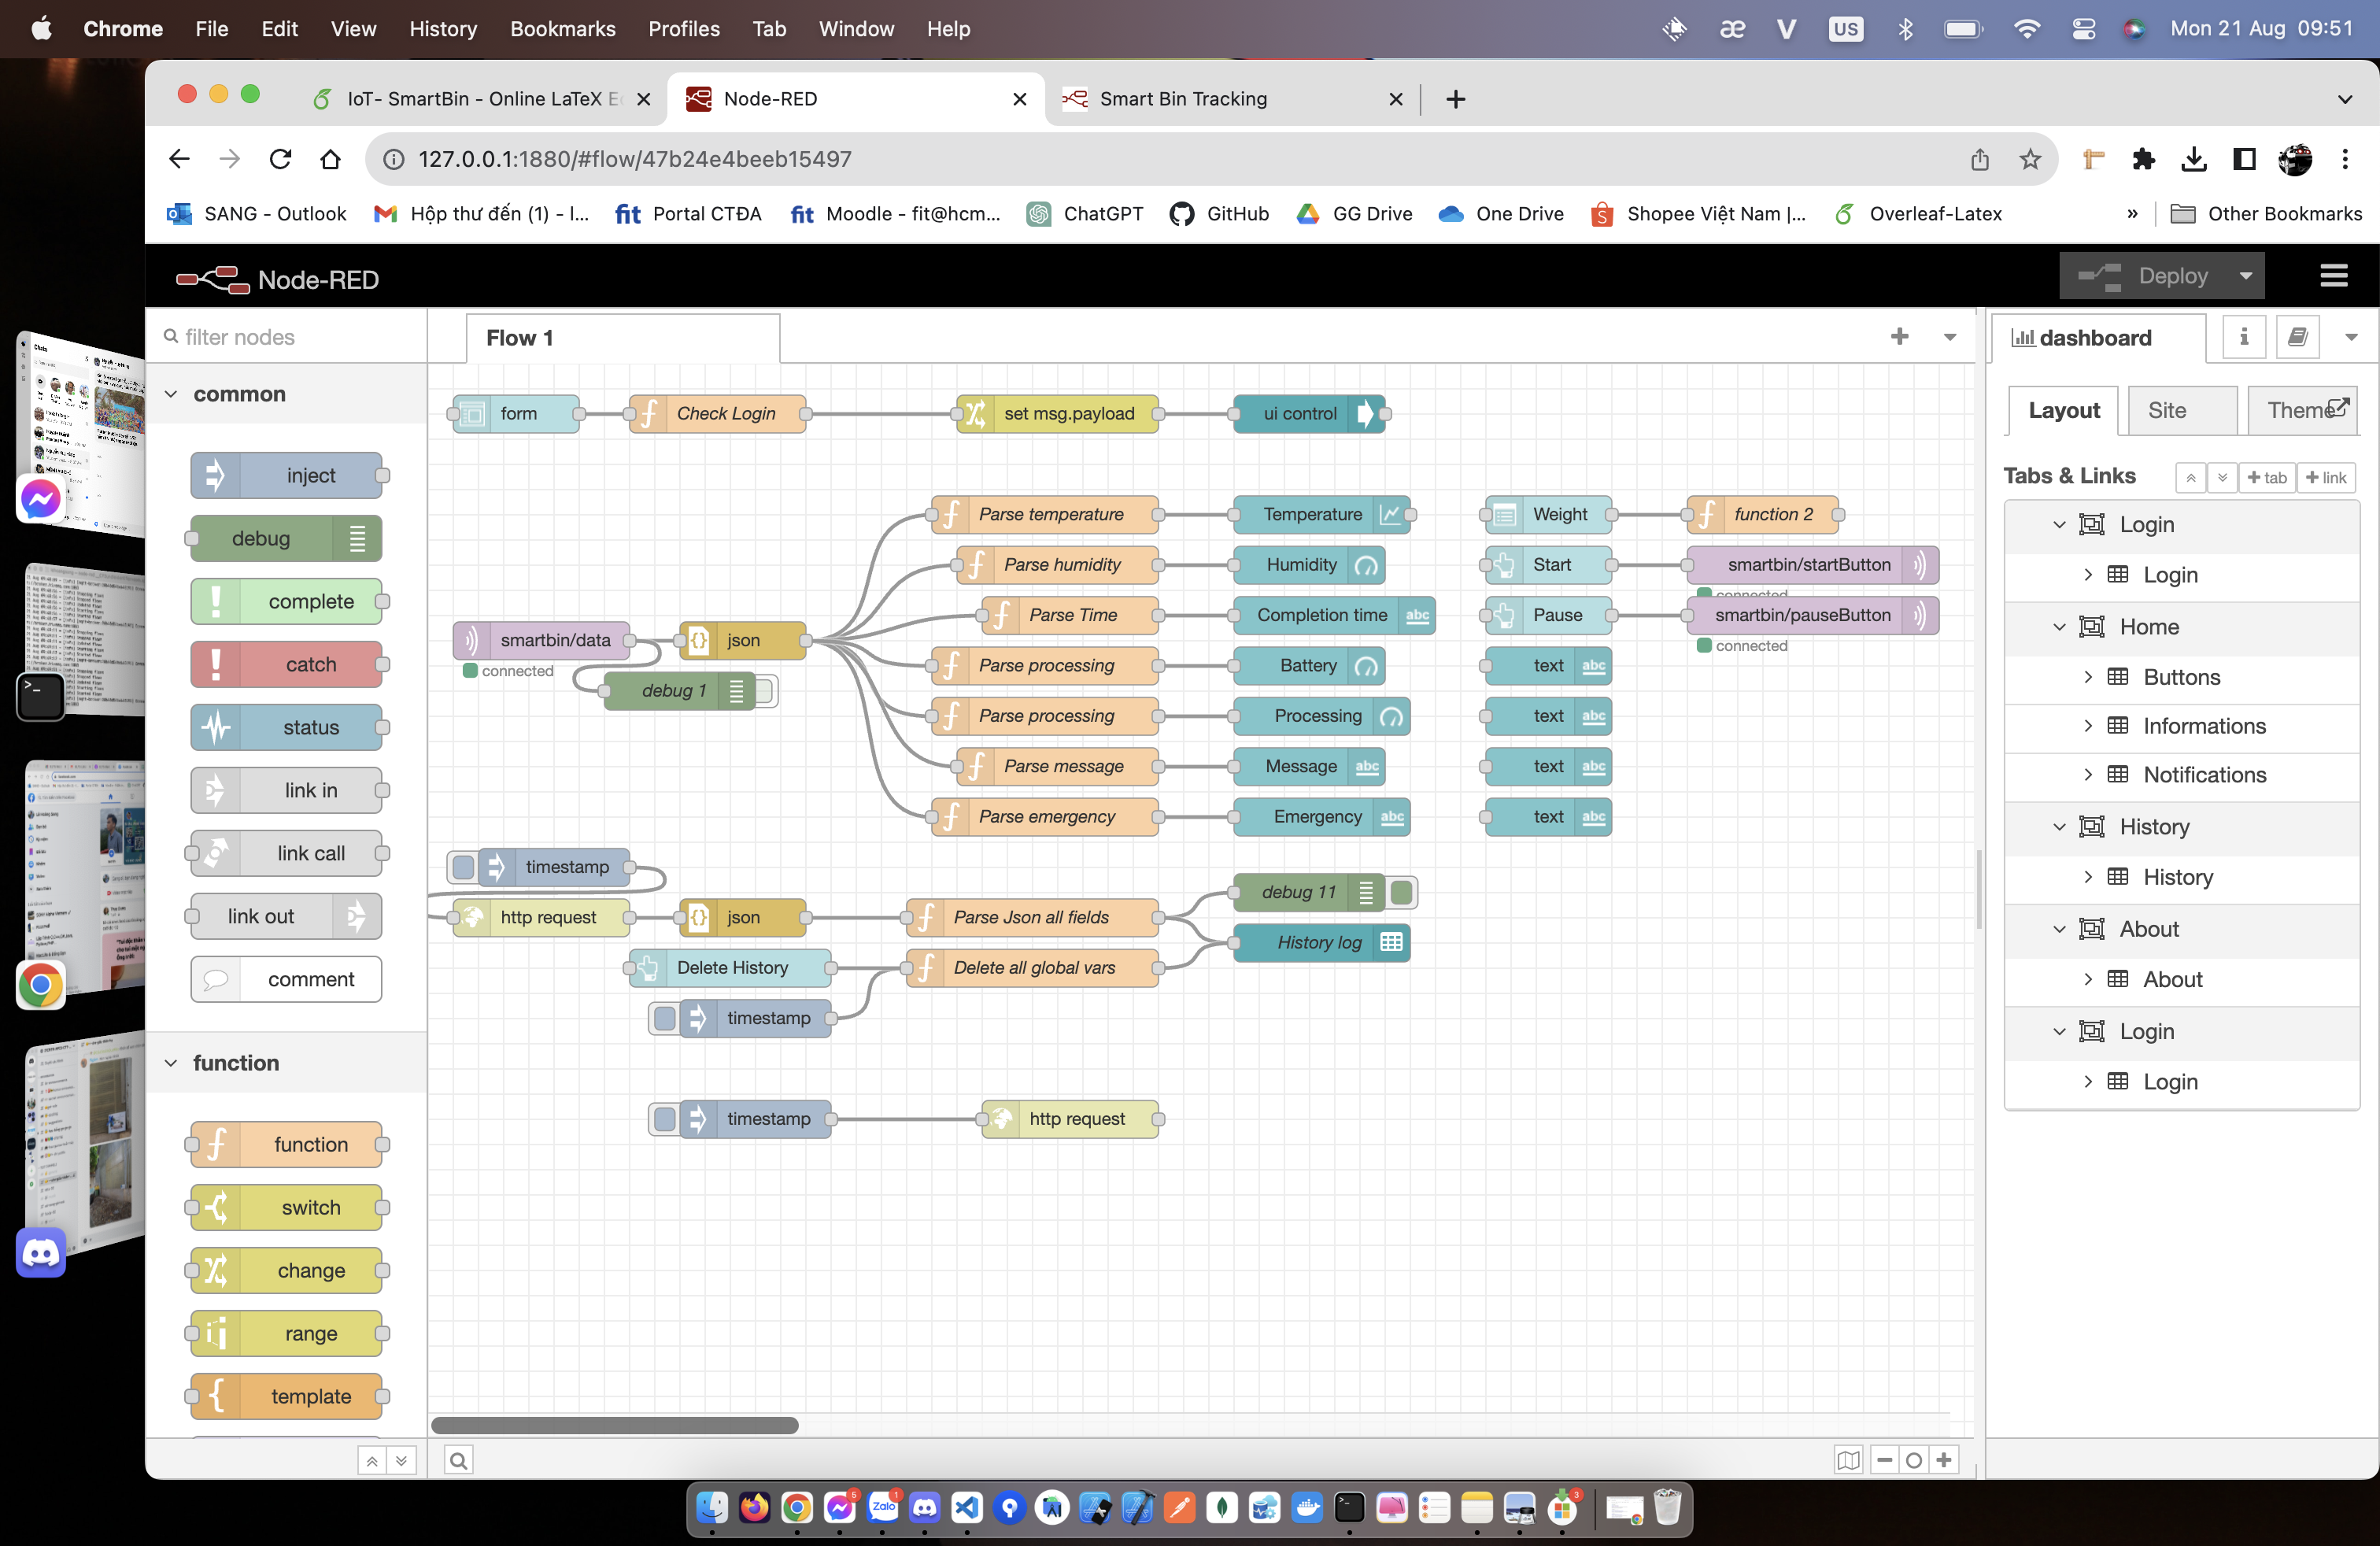
\includegraphics[width=0.9\linewidth]{Node/node-red.png}
            \caption{Hình ảnh minh họa Node-Red.}
        \end{subfigure}
\end{figure}
\pagebreak
\subsection{Mô tả quá trình hoạt động của website}
\subsubsection{Luồng nhận dữ liệu:} 
        \begin{itemize}
            \item Đầu tiên, website sẽ nhận một JSON từ mạch điện gửi lên, gồm các thuộc tính:
            \begin{lstlisting}
    var jsonDoc = {
        "temperature": 25,
        "humidity": 60,
        "start_time": "2023-08-1",
        "completion_time": "2023-08-18",
        "processing": 55,
        "message": "Processing is underway.",
        "emergency": "Nothing.",
        "battery": 80
      };\end{lstlisting}
            \item Các thông tin trên sẽ được lấy ra và hiển thị trên website thông qua các node ở tab Home, giúp người sử dụng có thể theo dõi từ xa các thông số (được thể hiện trực quan như hình bên trên) của quá trình ủ tại nhà.
        \end{itemize}
        
\subsubsection{Điều khiển thiết bị:} 
        \begin{itemize}
            \item Website cung cấp cho người dùng các nút Start/ Pause và chọn chế độ khối lượng rác bỏ vào.
            \item Cụ thể hơn, khi người dùng muốn kích hoạt thùng rác từ xa thì chỉ cần chọn chế độ khối lượng rác (ít, vừa, đầy) và ấn Start. 
            \item Ngược lại, người dùng có thể ấn Pause để tạm dừng quá trình ủ rác (trong trường hợp có sự cố).
            \item Khi người dùng ấn nút Start, website sẽ gửi về cho mạch điện một trong ba số: 0, 1, 2 đại diện cho việc khởi động với các khối lượng ít, vừa, đầy tương ứng.
            \item Khi người dùng ấn Pause, website sẽ gửi về mạch điện số 4, báo hiệu tín hiệu dừng.
        \end{itemize}

\subsubsection{Đọc dữ liệu từ Cloud ThingSpeak:} 
        \begin{itemize}
            \item Mạch điện sẽ gửi thông tin về thời gian, các sự số khẩn cấp của quá trình ủ lên Cloud. Thông qua đó, website sẽ lấy các dữ liệu đó và hiển thị cho người dùng về thông tin các quy trình ủ đã hoàn thành trước đây.
            \item Khi các dòng thông tin quá nhiều, người dùng có thể ấn nút Xóa lịch sử để xóa bớt các dòng hiển thị. Các dòng thông tin này được hiển thị bằng node Table, từ thư viện Table-UI.
            \item Node Timestamp sẽ lặp và gọi lại dòng  dữ liệu mới nhất sau vài ngày hoặc một tuần để cập nhật dữ liệu mới nhất từ Cloud.
            \item Cách lấy dữ liệu từ Cloud như sau: node sẽ gửi http request lên Cloud sau đó nhận được một data gồm các thuộc tính created\_at, start\_time, completion\_time, emergency. Các thuộc tính sẽ được đảm bảo được đóng gói thành JSON. Tiếp theo, hàm Parse Json all fields sẽ thực hiện push JSON mới vừa nhận vào list các JSON đã được lưu trong Flow trước đó (nếu có) để tạo thành một mảng các thông tin. List dữ liệu này sẽ được hiển thị trên tab History. 
            \item Để thực hiện việc xóa danh sách hiển thị lịch sử, ta chỉ việc gán lại mảng logs trong Flow là [] (mảng rỗng).
        \end{itemize}



\section{HƯỚNG PHÁT TRIỂN THÊM}
\textbf{Đây là những hướng đi có thể áp dụng được trong phiên bản cải tiến thêm của máy mà nhóm đã đút kết được: }
\begin{itemize}
    \item Cần phát triển máy hoạt động sao cho công suất lớn hơn đáp ứng nhu cầu phong phú của nhiều người.
    \item Phát triển nhiều hơn các chức năng, chế độ trên cả website lẫn thiết bị.
    \item Nghiên cứu chu kỳ hoạt động của từng loại rác khác nhau đẻ tìm điều kiện tối ưu.
    \item Cần phân tích thành phần hóa học sản phẩm hoặc kiểm soát đầu vào để sản phẩm được sử dụng hiệu quả.

\end{itemize}

\section{CÁC TÀI LIỆU THAM THẢO}
\begin{itemize}
    \item \href{https://www.iqhome.org/uploading-sensor-data-to-thingspeak-with-node-red}{Uploading sensor data to ThingSpeak with Node-RED}
    \item \href{https://stevesnoderedguide.com/working-with-json-data-node-red}{Working with JSON Data And JavaScript Objects in Node-Red}
    \item \href{https://www.youtube.com/watch?v=p74GGc5CZoc}{Hướng dẫn cài đặt Node-Red \& Làm quen với Node-red}
    \item \href{https://ohstem.vn/lp-courses/lap-trinh-arduino/lap-trinh-arduino-phan-ket-noi-wifi/}{Hướng dẫn lập trình Arduino kết nối wifi}
    \item \href{https://www.emuniv.com/products/che-pham-vi-sinh-vat-huu-hieu}{Giới thiệu chế phẩm vi sinh Emuniv}
\end{itemize}
\vspace{100pt}

\begin{center}
    \Large{Hết!}
\end{center}

\end{document}       